% Research proposal: Investigate, Recommend or Escalate: A Rule-Constrained Reinforcement Learning
% Agent for IT Incident Triage under Ambiguous Evidence
%
% Built on the department template _U_Proposal_Report_template_2026_CS_DS_Undergraduate.zip
% (same preamble, title page, preliminary pages, chapter and appendix order).
% Build from this folder:   ..\..\tools\tectonic.exe Opol_Charis_Research_Proposal.tex
% References come from ../thesis/citations/references.bib and proposal_extra.bib;
% figures from ../thesis/images/ and images/.

\documentclass[12pt]{report}
\usepackage{appendix}
\usepackage[utf8]{inputenc}
\usepackage{graphicx}
\usepackage{color}
\usepackage[table]{xcolor}
\usepackage{longtable}
\usepackage[paper=a4paper,bottom=2cm,footskip=0.25cm,top=2cm,headsep=0.25cm,rmargin=2cm,lmargin=2cm]{geometry}
\usepackage{tabularx}
\usepackage{xltabular}
\usepackage{booktabs}
\usepackage{float}
\usepackage[parfill]{parskip}
\usepackage{enumerate}
\usepackage{enumitem}
\usepackage{amssymb}
\usepackage{multirow}
\usepackage{tikz}
\usetikzlibrary{positioning}
\usepackage{cite}
\usepackage[hyphens]{url}

\usepackage{hyperref}
\usepackage{mathtools}
\hypersetup{
    colorlinks=false,
    linktoc=all,
    linkcolor=blue,
}

\usepackage{soul}

\setcounter{secnumdepth}{3}    % Number subsubsections in the chapters
\setcounter{tocdepth}{3}       % Put subsubsections in the table of contents

\graphicspath{{images/}{../thesis/images/}}
\emergencystretch=1.5em
\newcolumntype{L}{>{\raggedright\arraybackslash}X}
\newcolumntype{P}[1]{>{\raggedright\arraybackslash}p{#1}}
\newcommand{\cellyes}{$\checkmark$}
\newcommand{\cellpart}{$\circ$}
\newcommand{\cellno}{--}
\newcommand{\todo}[1]{\textcolor{red}{#1}}

%%%% Student data fields %%%%
\newcommand\theResearchTopic{\textit{Investigate, Recommend or Escalate: A Rule-Constrained Reinforcement Learning Agent for IT Incident Triage under Ambiguous Evidence}}

\newcommand\theStudentName{\textit{OPOL CHARIS}}
\newcommand\theStudentRegNo{\textit{S24B23/003}}
\newcommand\theStudentNo{\textit{B29654}}
\newcommand\theStudentEmail{\textit{charisopol@gmail.com}}
\newcommand\theStudentPhoneNo{\textit{0765821211}}

\newcommand\theSpecializationTrack{\textit{Artificial Intelligence and Robotics}}

\newcommand\thePrimaryAdvisor{\textit{\todo{IAN RAYMOND OSOLO}}}
\newcommand\theSupervisor{\thePrimaryAdvisor}

\newcommand\theProgrameAward{Bachelor of Science in Computer Science}
\newcommand\theTheDocumentType{proposal}
\newcommand\theFinalOutputDocument{Degree}

\newcommand\theFaculty{Faculty of Engineering Design \& Technology}
\newcommand\theDepartment{Department of Computing \& Technology}

\newcommand\theVersionDate{\textit{\todo{[Enter Version Date]}}}

%%%%%=====================. %%%%

\newcommand\makLogo{
\includegraphics[scale=.3]{images/logos/UCU-Logo.png}}


\pagenumbering{roman}
\begin{document}
    %%---- Title page
    \begin{titlepage}
        \centering
        \makLogo  \\
         \theDepartment \\
    	\vspace{1cm}
        \Large{
            \theResearchTopic \\

            \vspace{.5cm}
            \textit{By}\\
            \vspace{.5cm}
            \theStudentName\\

            Reg No: \theStudentRegNo, Student No: \theStudentNo  \\
            E-mail: \theStudentEmail, Phone No:  \theStudentPhoneNo\\

            \vspace{1cm}

            A \theTheDocumentType~submitted to the \theFaculty~for the study leading to the \theFinalOutputDocument~in partial fulfilment of the requirements for the award of \textbf{\theProgrameAward}~of Uganda Christian University \\

            \vspace{1cm}

            SPECIALIZATION TRACK: \theSpecializationTrack\\
              \vspace{1cm}
            \thePrimaryAdvisor \\

             \vspace{1cm}
            \theVersionDate \\
       }
    \end{titlepage}


%%%=== Preliminary pages ====
\chapter*{Declaration}
\label{pre:01-declaration}
\addcontentsline{toc}{chapter}{Declaration}
I, \theStudentName, declare to the best of my knowledge that the work in this \theTheDocumentType~is original and has not been submitted before to any university/institution. It is the result of my effort.

\vspace{1.5cm}

Signature: \line(1,0){8.0cm} \\

\vspace{1.5cm}
Date:	\line(1,0){8.0cm}\par


\chapter*{Ethical Generative AI Usage Declaration}
\label{pre:01b-AI-declaration}
\addcontentsline{toc}{chapter}{Declaration}
\begin{enumerate}[label=\Alph*.]
    \item \textbf{Declaring the use of AI in preparing this proposal}

        I, \theStudentName, declare that generative AI was used in preparing this \theTheDocumentType~only in the ways disclosed in Appendix~\ref{App:AI-use-declaration}: to review my arguments and suggest improvements to the clarity and structure of my work; to assist with the systematic literature review, including refining search strategies, reviewing literature and strengthening the discussion of research gaps; and to write and format LaTeX code for tables, generate some figures and improve the document layout. I evaluated every suggestion and output, and retained or modified it based on my own research and understanding.

        \vspace{1cm}

        Signature: \line(1,0){8.0cm}
        Date:	\line(1,0){4.0cm}\par
    \vspace{1cm}
    \item \textbf{Acknowledging the use of AI as a study buddy}

        Appendix~\ref{App:AI-use-declaration} gives the complete declaration of AI usage, including the tool used and the purposes for which it was used.
\end{enumerate}


\chapter*{Approval}
\label{pre:02-approval}
\addcontentsline{toc}{chapter}{Approval}
This~\theTheDocumentType~has been submitted for examination with approval of the following advisors/supervisor.\\

\textbf{\theSupervisor} \\
\theDepartment\\
\theFaculty\\
Uganda Christian University\\

\vspace{1.5cm}

Signature: \line(1,0){5.5cm}\par
\vspace{1.5cm}

Date:	\line(1,0){6.2cm}\par


\chapter*{Abstract}
\label{pre:03-abstract}
\addcontentsline{toc}{chapter}{Abstract}
When an IT incident is reported, the staff who receive it must decide what to do before they know its cause: investigate further, apply a likely fix, or pass the incident to someone better placed to resolve it. The first evidence is often incomplete, unreliable or consistent with more than one cause, yet most automated triage tools treat the decision as a single prediction from the incident report. They cannot ask for more evidence, cannot say that they are unsure, and do not check their suggestions against an organisation's operational rules.

This research proposes to design and evaluate a rule-constrained reinforcement learning agent that, for each incident, learns whether to request a diagnostic check, recommend a fix that the operational rules permit, or escalate the incident to a human expert. An independent rule-based safety mechanism checks every proposal, returns a blocked proposal to the agent once, and escalates the incident if the second proposal is also blocked. The agent will be trained and evaluated in a simulation built from incident scenarios elicited from the Directorate of University ICT Services at Uganda Christian University, in which missing, unreliable and overlapping evidence can each be controlled, and compared with six baseline policies on decision quality, investigation efficiency, escalation behaviour and constraint compliance. A systematic review of 34 studies, conducted for this research, found no published agent that combines these three decisions for IT service incidents under explicit rules.


\chapter*{Dedication}
\label{pre:04-dedication}
\addcontentsline{toc}{chapter}{Dedication}
I dedicate this research proposal to my father, Rev.\ Canon Dr Samuel Opol.


%=======================
\tableofcontents
 %=======================


\chapter*{Acknowledgments}
\label{pre:06-acknowledgments}
\addcontentsline{toc}{chapter}{Acknowledgments}
I want to thank God Almighty for strengthening me to work on this proposal and for the direction this research has taken. His grace started the good work, and grace will finish it.

I also thank my parents, Rev.\ Dr Samuel Opol and Margaret Opol, for the support they have given me, rallying me on when things got tough.

I thank Rebecca Kangabe, the Director of University ICT Services, Kenneth Musasizi, the Technical Lead at University ICT Services, and Simon Lubambo, the Senior Developer at University ICT Services, for their support of this research.

Finally, I thank Emmanuel Isabirye for redirecting my research.

%%==End of preliminary pages


%%%%======================== Beginning of Chapters
\chapter{Introduction}
\label{ch:chapter-01}
 %%%%========================
 \pagenumbering{arabic}
 \renewcommand{\arraystretch}{1}
 %%%=========================
\section{Background}

Organisations depend on IT services that are expected to remain available, and incident management is the process that restores those services when they fail. Chen et al.\ describe it as detecting a service problem, creating an incident, determining its cause, restoring the service, and capturing knowledge to prevent a recurrence~\cite{chen2020}. Incident triage is the stage at which a reported incident is assessed and directed towards resolution~\cite{chen2020,remil2024}. It is a set of decisions made before the cause of the incident is known.

These decisions are difficult because the evidence available when they are made is often incomplete or conflicting. In a two-year study of incident management at Microsoft, Chen et al.\ found that distinct problems can produce similar symptoms, so that the symptoms alone may not identify the responsible team, and incidents are reassigned several times as a result~\cite{chen2020}. Remil et al.\ note that data in real IT environments is commonly noisy and incomplete~\cite{remil2024}. At the Directorate of University ICT Services (UIS) at Uganda Christian University, incidents reach developers through user tickets that are vetted and assigned, and application errors are diagnosed from system logs and a monitoring dashboard. An initial interview with a senior developer of the Directorate in October 2026 described this process and identified the application programming interface logs as the most informative source of evidence.

Reinforcement learning (RL) offers a way to treat triage as a sequence of decisions. In RL, an agent learns a policy, which is a rule for choosing actions, by acting in an environment and receiving rewards that reflect the consequences of its actions~\cite{sutton2018}. When the agent cannot observe the true state, it can choose actions for the information they yield, and weigh the cost of that information against its value~\cite{kaelbling1998}. Under this framing, an agent faced with an ambiguous incident can gather more evidence, recommend a fix, or hand the incident to a person.

\section{Problem Statement}

IT support teams must decide how to handle an incident before they know its cause, because its symptoms are often not enough to identify the problem: distinct problems can produce similar symptoms~\cite{chen2020}. A member of IT staff facing such an incident can investigate further, apply a likely remedy, or pass the incident to someone better placed to resolve it, and each choice has a cost. Further investigation takes time, since engineers often need a long time to identify an incident's root cause~\cite{chen2020}. A wrong remedy can reduce availability instead of restoring it~\cite{alauthman2026}, and an incident sent to the wrong team is reassigned, which prolongs the downtime~\cite{chen2020}. Escalation draws on the limited attention of the people who receive it, and when they are overloaded, responses are delayed and significant incidents are missed~\cite{kovtun2026,turan2026}.

Existing automated approaches address parts of this decision but not the choice among its options. Triage models commonly produce one prediction per incident report and are evaluated with classification metrics~\cite{chen2020,remil2024}, so they cannot ask for more evidence and cannot say that they are unsure. Reinforcement learning has been applied to incident response and investigation, mostly in cybersecurity~\cite{dunsin2025,hammar2025,hammar2026belief}, and a few studies of security alert triage let an agent gather evidence and then escalate or defer an alert to an analyst~\cite{sahin2026,kovtun2026}. Their agents close or escalate alerts, however, and do not recommend a fix that changes the affected system. A systematic review of 34 studies, conducted for this research, found escalation to a person in only seven of them, and only three that report what happens when a rule mechanism blocks a decision. A reward penalty alone does not ensure that an agent respects an organisation's operational rules, because penalising an action does not guarantee that the agent never selects it~\cite{konighofer2025}.

As a result, the reviewed literature contains no evaluated agent for IT service incidents that learns when to investigate, when to recommend a permitted fix and when to escalate, with its proposals checked against explicit operational rules, and no evidence on how such an agent behaves as the evidence becomes more ambiguous. This research seeks to address that gap. It does not claim that constraining a learned incident-handling agent is new; its contribution lies in the decision it studies, the setting, and the way the result is evaluated.

\section{Research Objectives}

The general objective of this study is to design and evaluate a rule-constrained reinforcement learning agent for ambiguity-aware IT incident triage that learns when to gather additional diagnostic information, recommend permitted actions, or escalate incidents to a human expert. It is guided by the following specific objectives.

\subsection{Scenario Model and Simulated Environment:}

To build a simulated triage environment from a scenario model of about 15 causes, 20 diagnostic checks and 10 operational rules elicited from the Directorate and reviewed by its staff, in which an agent can request diagnostic information, recommend permitted actions or escalate incidents, and in which missing, unreliable and overlapping evidence can each be set independently. This objective addresses how ambiguous triage scenarios can be represented in a controlled environment.

\subsection{Rule-Constrained Agent:}

To train a deep Q-network agent that chooses among requesting checks, recommending fixes and escalating, under an independent rule-based safety mechanism that returns a blocked proposal to the agent once and escalates the incident if the second proposal is also blocked, so that no prohibited action is executed, and to repeat the training with proximal policy optimisation as a robustness check on the choice of learning algorithm. This objective addresses how reinforcement learning can support the three decisions and how a rule mechanism affects the agent's decisions.

\subsection{Evaluation against Baselines and under Ambiguity:}

To evaluate the agent against six baseline decision policies on decision quality, investigation efficiency, escalation behaviour and constraint compliance, and to measure how its accuracy and its mix of investigating, recommending and escalating change across controlled levels of missing, unreliable and overlapping evidence. This objective addresses how the approach compares with simpler policies and how robust it is as the evidence becomes more ambiguous.

\section{Research Questions}

This study will answer the following research questions:

\begin{enumerate}
\item How can ambiguous IT incident scenarios, built from the causes, diagnostic checks and operational rules of the Directorate, be represented in a simulated environment in which missing, unreliable and overlapping evidence can each be controlled?
\item How effectively can a reinforcement learning agent learn when to request diagnostic information, when to recommend a permitted fix, and when to escalate an incident to a human expert, and do the findings hold when the deep Q-network is replaced by proximal policy optimisation?
\item How does a rule-based safety mechanism, which returns a blocked proposal to the agent once and escalates the incident after a second block, affect the agent's compliant success, its rate of blocked proposals and its decisions, compared with an agent without the mechanism and an agent that learns the rules only from a reward penalty?
\item How does the agent compare with the selected baseline decision policies, and how do its accuracy and its mix of investigating, recommending and escalating change as the evidence becomes more ambiguous?
\end{enumerate}

\section{Research Hypotheses}

This study will test the following hypotheses. The criteria by which each is judged supported or not supported are stated in Section~\ref{sec:criteria}.

\begin{description}[labelwidth=2.5em, leftmargin=3.2em, labelindent=0.5em]
\item[H1:] At the base level of ambiguity, the agent will achieve a higher resolution accuracy than the initial-symptom, scripted-checklist and always-escalate baseline policies, with a mean investigation cost no higher than that of the scripted checklist.
\item[H2:] The agent with the safety mechanism will achieve a higher compliant success rate, the share of incidents resolved correctly without any prohibited action taking effect, than the unconstrained and penalty-only agents.
\item[H3:] The agent's response to ambiguity will depend on its source:
\begin{description}[labelwidth=3.2em, leftmargin=3.6em]
\item[H3a:] as more evidence goes missing, it will escalate more incidents, without requesting more checks, since unavailable checks cannot be requested;
\item[H3b:] as evidence becomes less reliable, it will request more checks before deciding and recommend fixes on fewer incidents;
\item[H3c:] as the evidence for different causes overlaps more, it will request more checks and escalate more incidents.
\end{description}
\end{description}

That the safety mechanism prevents every prohibited action is not a hypothesis, because it holds by construction (Equation~\eqref{eq:mechanism}). It is checked as a verification of the implementation: the executed-violation rate must be zero on every evaluation incident in which the mechanism is active.

\section{Justification}

This research is justified by a decision that IT support teams face routinely and that existing automated approaches represent only in part. The literature shows that incident evidence is often insufficient to identify the cause~\cite{chen2020}, and that automation in AIOps mainly stops at triage or the recommendation of solutions, with automatic execution limited and unverified~\cite{zhang2025}. Reinforcement learning and explicit rules compensate for each other's weaknesses: the learner can judge when further investigation is worth its cost, which fixed rules handle poorly, and the rules give an assurance about prohibited actions that a learned policy cannot~\cite{alshiekh2018}. Keeping the rules in a mechanism separate from the learner also makes them readable and changeable by IT staff.

The study is feasible and low-risk because it is carried out entirely in simulation. Simulation allows the level of ambiguity to be controlled and experiments to be repeated, without acting on any live system of the university. Working with the Directorate grounds the simulated scenarios and rules in the practice of an operating IT support unit. The study also supports the use of artificial intelligence in Uganda's public and institutional IT services, which Appendix~\ref{App:research-allignment-with-national-and-global-agenda} relates to the programme specialisation and to national and global development goals.


\chapter{Literature Review}
\label{ch:chapter-02}
\section{Literature Review Plan}
\label{ch02:sec:plan}

The review was planned around the decision this research studies: what an agent should do with an IT incident whose cause is uncertain. It drew on two sources. The first was a core set of publications on AI for IT operations (AIOps), safe reinforcement learning and learning to defer, collected while the problem was being defined. The second was a systematic review, reported following the PRISMA 2020 guideline~\cite{page2021}, which searched Scopus, the ACM Digital Library and IEEE Xplore, with the Scopus and ACM searches limited to publications from 2015 to 2026, and included 34 studies that apply reinforcement learning or sequential decision-making to IT or security incident handling. The search strings are given in Appendix~\ref{App:scopus-search-strings} and the flow of records in Appendix~\ref{App:figures-other}.

The literature is discussed chronologically, in the order in which the strands developed: the foundations of safe reinforcement learning, then information gathering and deferral, then the prediction-based approaches of AIOps, then reinforcement learning for incident handling, and finally the recent studies that begin to combine these strands. For each approach the review states what it does, what evidence supports it and where it falls short, and then judges it against five requirements that an agent for IT incident triage at a university IT directorate must meet:

\begin{enumerate}[label=\textbf{R\arabic*.}]
\item \textbf{Sequential decisions:} the agent decides step by step, and each step can change what it knows.
\item \textbf{Costly investigation:} the agent can request a diagnostic check and weigh what the check costs against what it may reveal.
\item \textbf{Remedy or hand-over:} the agent can recommend a fix that changes the affected system, or hand the incident to a human expert.
\item \textbf{Operational rules:} every proposed action is checked against the organisation's rules, and a prohibited action is never carried out.
\item \textbf{Ambiguous evidence:} the agent stays reliable as the evidence becomes missing, unreliable or consistent with several causes.
\end{enumerate}

\section{Review of Approaches to Incident Triage}
\label{ch02:sec:review}

\subsection{Foundations of Safe Reinforcement Learning (2015--2018)}

These methods keep a learning agent from taking prohibited actions, and they are the source of the rule mechanism in this study (R4).

\begin{itemize}
\item \textbf{Constrained optimisation (2015--2017):} García and Fernández divided safe reinforcement learning into methods that change the optimisation criterion and methods that change exploration with external knowledge~\cite{garcia2015}. Constrained policy optimisation, from the first group, bounds the expected cumulative cost of a policy and guarantees near-constraint satisfaction at every training iteration~\cite{achiam2017}. Its strength is that safety is built into training rather than added afterwards. Its weakness is that the guarantee holds on average: an expected-cost bound does not enforce a rule that must hold at every step~\cite{zhao2023}, and a reward penalty discourages an action without preventing it~\cite{konighofer2025}. The rules of an IT directorate are not averages; a rule such as ``do not restart a production service without approval'' must hold on every incident, so this approach cannot meet R4 on its own.

\item \textbf{Shielding (2018 onwards):} Alshiekh et al.\ introduced a shield, a separate component that checks each action the agent proposes and blocks or replaces it when it would violate a specification, so that safety holds during both learning and deployment while the agent is restricted as little as possible~\cite{alshiekh2018}. For this study the main strength is the separation: the rules sit outside the learner, where IT staff can read and change them. Three weaknesses remain. The shield is computed from an abstraction of the environment's dynamics~\cite{alshiekh2018}, and shields that need a full model of the environment cannot be applied where no such model exists~\cite{yang2023}. A shield that silently replaces actions can hinder learning, because the agent does not know it was overridden~\cite{yang2023}. And shields have been demonstrated mainly in control tasks and games~\cite{alshiekh2018,konighofer2025}, not on the rules of IT operations. The rules of an IT directorate are conditions on the proposed action and the evidence gathered so far, so they can be checked without a model of how incidents evolve, but what happens to a blocked action has to be designed for this setting rather than borrowed.
\end{itemize}

Constrained optimisation shows that a penalty alone cannot meet R4, and shielding shows how R4 can be met. Neither addresses investigation, hand-over or ambiguous evidence.

\subsection{Information Gathering and Deferral (2018--2023)}

These methods let a model delay or hand over its decision, the two options that prediction-only triage lacks (R2 and R3).

\begin{itemize}
\item \textbf{Learning to defer (2018):} Madras et al.\ trained a model that can pass a decision to an external decision-maker and that accounts for the biases of that decision-maker; deferring made the combined system both more accurate and fairer, even when the human was inconsistent~\cite{madras2018}. Joshi et al.\ later extended deferral to sequential settings~\cite{joshi2023}, and selective prediction gives a model the related option to abstain when its confidence is low~\cite{geifman2019}. The strength of this line is that handing over is learned rather than set by a fixed threshold, and it is judged by how well the human and the model perform together. Its weakness for incident triage is that the model can only decide or hand over; it cannot ask for more evidence first. Madras et al.\ evaluated single classification decisions on recidivism and health datasets~\cite{madras2018}, where no further evidence can be collected. Applied to IT incidents, deferral alone would hand over incidents that one more check could have resolved.

\item \textbf{Information gathering (2019):} Janisch et al.\ trained an agent to acquire costly features one at a time before it classifies~\cite{janisch2019}, building on the principle that, under partial observability, an action may be chosen for the information it yields~\cite{kaelbling1998}. Its strength is that investigation is treated as a decision with a cost (R2), which is close to how IT staff work through diagnostic checks. Its weakness is the mirror image of deferral: the agent can look further or decide, but it cannot hand over, so when the evidence stays ambiguous it must still commit to an answer.
\end{itemize}

The two lines complement each other. Each supplies one of the options this study needs, neither supplies both, and neither checks its decisions against operational rules.

\subsection{Triage as Prediction in AIOps (2020--2025)}

These methods treat triage as the prediction of a label from the incident report.

\begin{itemize}
\item \textbf{Incident management at scale (2020):} Chen et al.\ conducted an empirical study of more than two years of incident management at Microsoft~\cite{chen2020}. Its strength is its evidence: drawn from real operations, it shows that distinct problems can produce similar symptoms, so that incidents are reassigned several times, which is the ambiguity this study simulates. The remedy it describes, however, is a recurrent model that predicts the responsible team from the incident text~\cite{chen2020}. Such a model makes one prediction per incident; when the text is ambiguous it still names a team, and the reassignments the study documents are the cost of naming the wrong one.

\item \textbf{AIOps surveys (2024--2025):} Remil et al.\ catalogued the methods for classifying, prioritising and assigning incidents, and criticised the reliance on classification metrics that ignore the cost of a wrong action~\cite{remil2024}. Zhang et al.\ observed that language-model assistants extended this work to diagnosis and mitigation suggestions, but that automation mainly stops at triage or recommendation~\cite{zhang2025}. The surveys are valuable as maps of the field and for the measurement problem they identify. The methods they survey, though, return an answer for every report and are scored on how often that answer is right. They cannot state that more evidence is needed or that a person should decide (R2, R3), and accuracy says nothing about whether a recommended action was permitted (R4).
\end{itemize}

This group supplies the problem and the evidence for it, but not a model of the decision. It corresponds to the single-prediction baseline against which this study's agent is compared.

\subsection{Reinforcement Learning for Incident Handling (2023--2026)}

These studies treat incident handling as a sequence of decisions (R1).

\begin{itemize}
\item \textbf{Root cause analysis (2023):} Wang et al.\ used hierarchical reinforcement learning to decide which questions to put to engineers when building a service dependency graph for Microsoft's microservice systems, reducing the number of queries needed from $O(N^2)$ to $O(1)$~\cite{wang2023hrlhf}. Ding et al.'s TraceDiag learned to prune the dependency graph before analysis and was deployed in production at Microsoft~\cite{ding2023}. Both treat investigation as a decision with a cost (R2), and both were built on real production systems, which few studies in this review achieve. Their goal, however, is to locate a root cause, not to decide what to do about it: neither recommends a remedy, checks one against rules, or decides whether a person should take over. Both also rely on the dependency graphs and traces of large microservice systems, whereas the Directorate diagnoses errors from API logs and a monitoring dashboard.

\item \textbf{Security incident response (2025--2026):} Dunsin et al.\ trained an agent to conduct a malware investigation step by step, aiming to shorten post-incident forensic investigations, and evaluated it in simulated scenarios~\cite{dunsin2025}. Hammar and Li planned incident responses while holding a belief over the model of the incident itself, relaxing the usual assumption that the system model is known, and bounded the errors this introduces~\cite{hammar2025}. Hammar et al.\ adapted response policies to changes in the system without repeating the offline optimisation~\cite{hammar2026belief}. The Hammar studies are the strongest in this group on R5: on the CAGE-2 benchmark, and for the 2026 study also on a testbed, they outperformed earlier methods in robustness to an inaccurate model~\cite{hammar2025,hammar2026belief}. Their weaknesses for this study are twofold. Their agents choose among responses or investigative steps, but none can hand the incident to a person (R3), and none checks its actions against an organisation's rules (R4). Their environments also model cyberattacks, in which an adversary drives the incident, whereas the IT service incidents in this study arise from faults and misconfigurations.
\end{itemize}

This group shows that reinforcement learning can handle investigation and response as sequential decisions. In every study, however, the decision ends with the agent: none passes an incident to a person or respects operational rules.

\subsection{Recent Combinations (2025--2026)}

The most recent studies begin to combine the strands above, mostly in security operations.

\begin{itemize}
\item \textbf{Gathering evidence and escalating in alert triage:} Okafor trained offline agents that dismiss, investigate or contain security alerts, with escalation to analysts fixed by design~\cite{okafor2026}. Its strength is methodological: it avoids unsafe online exploration, removes temporal leakage from the evaluation, and shows that F1 and ROC-AUC can hide degenerate policies~\cite{okafor2026}. Its weakness is its data: public intrusion datasets hold flow records rather than decisions, so its training episodes are reconstructed from flows~\cite{okafor2026}, and the escalation it reports was not learned. Sahin and Mert trained an agent that queries logs and threat intelligence before it escalates or closes an alert, with a separate conformal layer that defers uncertain alerts to an analyst while controlling the rate of missed threats~\cite{sahin2026}. This gives hand-over a statistical guarantee rather than a tuned threshold, the strongest treatment of R3 in the review, but the deferral sits outside the learned policy: the agent itself is not taught when handing over is worth its cost. Kovtun et al.\ learned a policy that chooses among shallow triage, deep analysis and deferral under analyst-capacity constraints, and theirs is the one study that reports decision quality, cost, escalation and compliance together~\cite{kovtun2026}. Its evaluation, like Okafor's, rests on public intrusion datasets, CIC-IDS2017 and UNSW-NB15~\cite{kovtun2026}. Across the three, the actions close, contain or escalate an alert; none recommends a repair to a failing service, which is the action an IT directorate most needs to check against its rules.

\item \textbf{Rule mechanisms in incident response:} Ravi et al.'s SAFE-HGX added a safety layer to a hierarchical multi-agent learner for intrusion response in industrial control systems, replacing blocked actions, and in simulated attack scenarios it learned faster and contained attacks more accurately than DQN and PPO baselines~\cite{ravi2025}. The cost was high: about 9 to 11 times as many false-positive actions as the PPO baseline, and 74 to 77\% higher operating cost~\cite{ravi2025}. An IT directorate is unlikely to accept that trade-off, since an unnecessary action on a live service can itself disrupt operations~\cite{okafor2026}. Singh's deterministic guard for cloud remediation hands an action to a human when it fails~\cite{singh2026}. In its ablation, removing the guard left the mean time to resolve almost unchanged (144~s against 142~s) but cut governance compliance from 99.9\% to 72.3\%~\cite{singh2026}, the clearest evidence in the review that a hard rule check need not slow resolution. The learning in Singh's framework, however, is confined to a reinforcement learning meta-orchestrator that weights the recommendations of other agents~\cite{singh2026}, so the study does not show how a learning agent behaves when its own proposals are blocked. Alauthman et al.\ proposed a shielded DQN agent with operator override for incident response in industrial control systems, but reported an evaluation plan and indicative findings rather than measured results~\cite{alauthman2026}; it shows that the design is plausible, not that it works. Of the 34 studies in the systematic review, only three say what happens to a blocked decision, and none lets the agent propose again.
\end{itemize}

These two groups have reached the design questions of this study from opposite sides. The alert-triage studies hand cases over but do not check remedies against rules; the rule-mechanism studies check actions against rules but do not learn when to hand over. Their results also disagree on what a rule mechanism costs: Ravi et al.\ found many more false actions, while Singh found no loss of speed.

\subsection{Evaluation and Robustness}

These studies show how such agents have been evaluated, and where the evaluations fall short.

\begin{itemize}
\item \textbf{Measures:} In the systematic review, 31 of 34 studies measure decision quality, but only five measure escalation behaviour and four constraint compliance; one study, Kovtun et al., reports all four kinds of measure, for SOC alert escalation~\cite{kovtun2026}. This matters because each measure on its own can be satisfied by a poor policy: an agent that escalates every incident never breaks a rule and never recommends a wrong fix, but it is of no use to the people it escalates to. A single metric can also hide a degenerate policy: Okafor found that F1 and ROC-AUC concealed agents that had collapsed into trivial detectors, which the Matthews correlation coefficient exposed~\cite{okafor2026}.
\item \textbf{Robustness:} Fifteen of the reviewed studies test their agents under changed conditions, and the methods that keep a belief over the hidden state degrade least~\cite{hammar2025,hammar2026belief}. Sahin and Mert show that deferral to analysts rises as the evidence degrades~\cite{sahin2026}. These tests vary the conditions as a whole; no reviewed study reports how the mix of investigating, acting and escalating changes as ambiguity increases, which is the behaviour that shows whether an agent recognises when it does not know enough.
\end{itemize}

Table~\ref{tab:comparison} compares the studies closest to this research against the capabilities it requires.

\begin{table}[H]
\centering
\caption{Comparison of the studies closest to this research. \cellyes~=~addressed; \cellpart~=~partly addressed; \cellno~=~not addressed.}
\label{tab:comparison}
\small
\setlength{\tabcolsep}{4pt}
\begin{tabular}{|p{3.4cm}|p{4.2cm}|c|c|c|c|c|}
\hline
\textbf{Study} & \textbf{Setting} & \textbf{Seq.} & \textbf{Info.} & \textbf{Rule} & \textbf{Esc.} & \textbf{Amb.} \\
\hline
Chen et al.~\cite{chen2020} & IT incident triage & \cellno & \cellno & \cellno & \cellno & \cellno \\ \hline
Wang et al.~\cite{wang2023hrlhf} & Root cause analysis & \cellyes & \cellyes & \cellno & \cellpart & \cellno \\ \hline
Dunsin et al.~\cite{dunsin2025} & Malware investigation & \cellyes & \cellyes & \cellno & \cellno & \cellno \\ \hline
Hammar and Li~\cite{hammar2025} & Security incident response & \cellyes & \cellno & \cellno & \cellno & \cellyes \\ \hline
Alauthman et al.~\cite{alauthman2026} & Industrial control incident response & \cellyes & \cellno & \cellyes & \cellpart & \cellno \\ \hline
Ravi et al.~\cite{ravi2025} & Industrial control incident response & \cellyes & \cellno & \cellyes & \cellno & \cellno \\ \hline
Okafor~\cite{okafor2026} & Security alert triage & \cellyes & \cellyes & \cellpart & \cellpart & \cellno \\ \hline
Sahin and Mert~\cite{sahin2026} & Security alert triage & \cellyes & \cellyes & \cellpart & \cellyes & \cellyes \\ \hline
Kovtun et al.~\cite{kovtun2026} & Security alert escalation & \cellyes & \cellpart & \cellpart & \cellyes & \cellno \\ \hline
Singh~\cite{singh2026} & Cloud operations remediation & \cellpart & \cellno & \cellyes & \cellpart & \cellno \\ \hline
\textbf{This study} & IT incident triage & \cellyes & \cellyes & \cellyes & \cellyes & \cellyes \\ \hline
\end{tabular}

\vspace{4pt}
\raggedright\footnotesize Seq.\ = sequential policy; Info.\ = information gathering; Rule = rule check; Esc.\ = human escalation; Amb.\ = varied ambiguity.
\end{table}

\section{Research Gaps}
\label{ch02:sec:gaps}

The approaches reviewed above each solve part of the triage decision, but no reviewed study combines them for IT service incidents. The most significant gap is in the decision itself: information-gathering studies let an agent choose between looking further and deciding, deferral studies let it choose between deciding and handing over, and the security alert-triage studies that join the two do not recommend a fix that acts on the system. No reviewed study trains one policy to choose among investigating, recommending a remedy and escalating for IT service incidents. The second gap concerns the rules: hard rule mechanisms have been measured in only two studies, their results point in opposite directions, and no reviewed study gives a blocked agent a second proposal or reports how often blocked proposals occur during training. The third gap concerns robustness: decision accuracy and the rate of deferral have been tested under degraded evidence, but not the mix of investigating, recommending and escalating as ambiguity rises. Underneath all three lies a gap in representation, since the available environments model cyberattacks and microservice faults, and none lets the ambiguity of IT service incidents be varied.

These gaps are stated for the literature reviewed. The systematic review searched three databases, limited its IEEE Xplore search to open-access records, did not carry out citation searching, and could not retrieve seven reports. The claim is that the reviewed literature leaves these questions open, not that they have never been examined.


\chapter{Methodology}
\label{ch:chapter-03}
\section{Overview}

To study how an agent should handle IT incidents whose cause is uncertain, this research adopts a design-and-evaluate approach~\cite{hevner2004}. It builds an artefact, a rule-constrained reinforcement learning agent together with the simulated environment in which it acts, and evaluates it in controlled experiments. The work proceeds in eight phases, shown in Figure~\ref{fig:pipeline}: specifying the problem, eliciting scenarios with the Directorate, building and validating the environment, encoding the rules, implementing the baselines, training the agents, running the experiments, and analysing the results.

\begin{figure}[H]
\centering
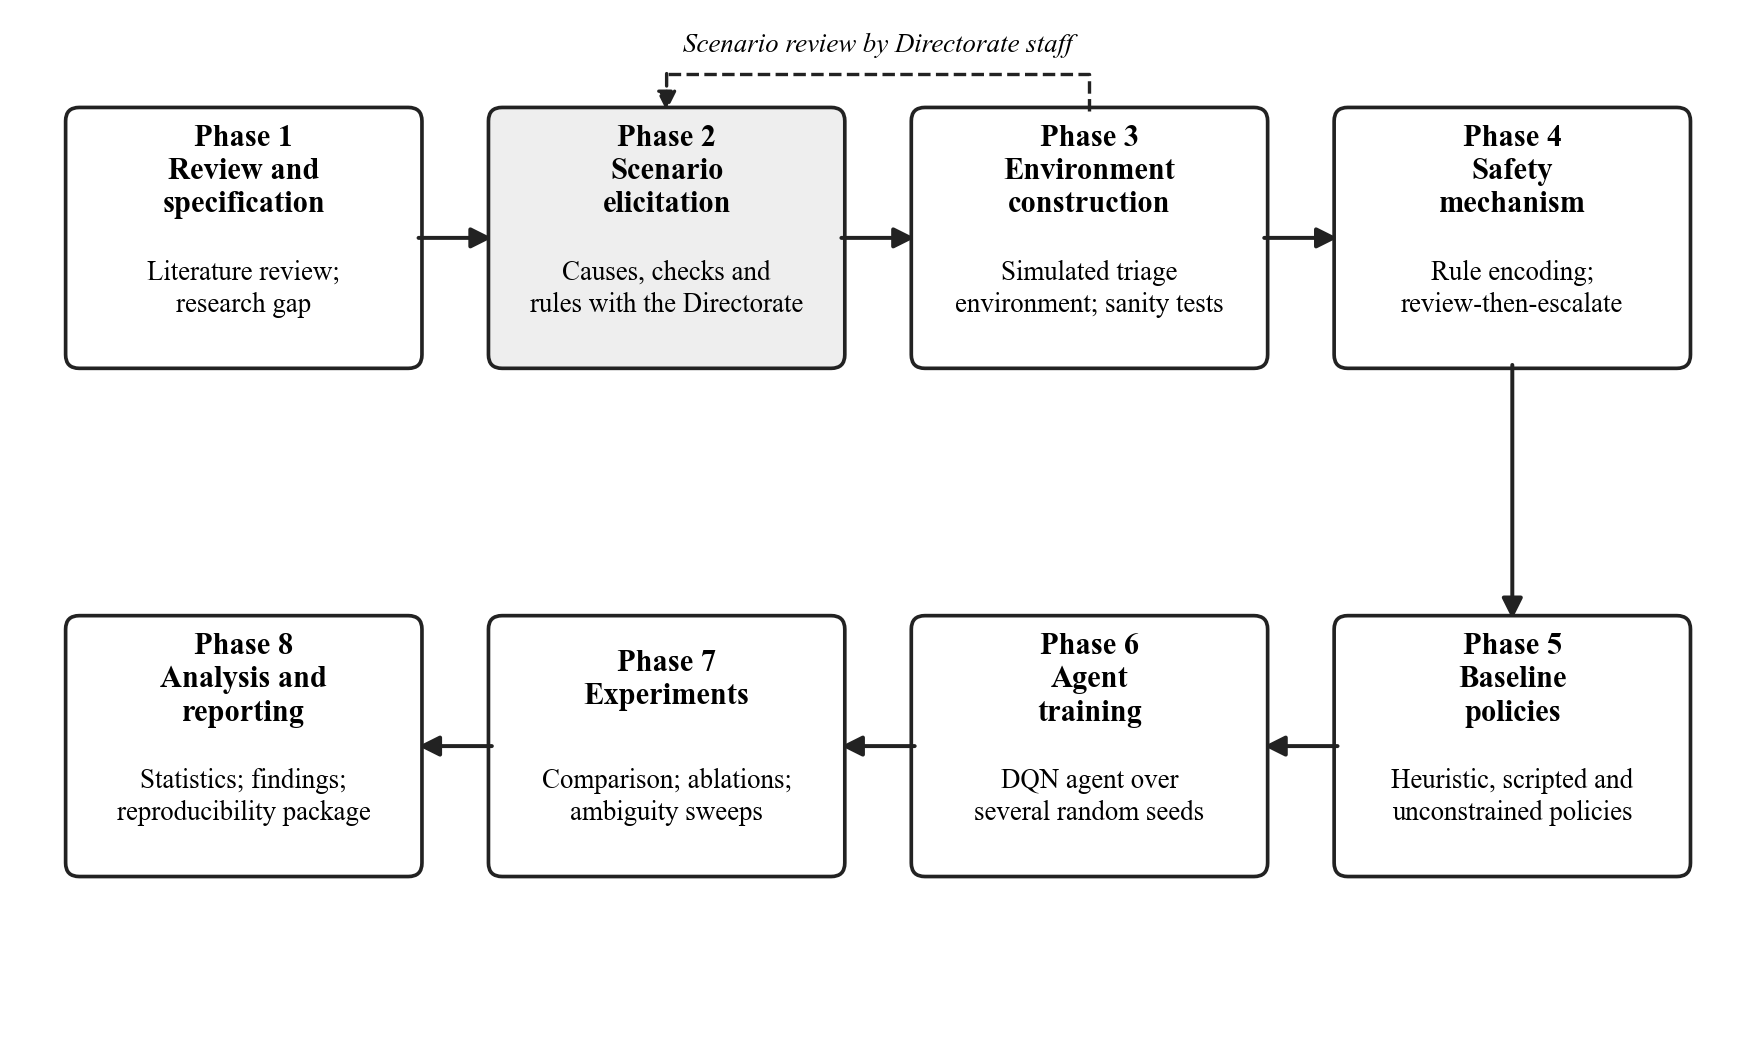
\includegraphics[width=\textwidth]{Figure_3_1_Research_Pipeline.png}
\caption{Research pipeline}
\label{fig:pipeline}
\end{figure}

The evaluation is conducted entirely in simulation, for two reasons. Realistic incident data is scarce and confidential~\cite{remil2024}, and simulation lets the level of ambiguity be set, held constant and varied, which live incidents would not allow. The agent is never connected to any system of the university. The framework will be implemented in Python, with the Gymnasium interface for the environment~\cite{towers2024} and the Stable-Baselines3 library for the learning algorithms~\cite{raffin2021}. No personal data, credentials or confidential details of the university's systems will enter the simulator, and staff participation will be voluntary and with consent.

\section{Data Collection}

The data for this research is a scenario model elicited from the Directorate of University ICT Services, not a dataset of incident records. The model will be elicited from Directorate staff using a structured workbook, and it will contain about 15 causes in four provisional categories (application and interface errors, authentication and access failures, database failures, and failures of infrastructure and external services), each with one correct fix; 20 diagnostic checks, such as an entry in the API logs, a value on the monitoring dashboard or the result of reproducing a failing request, each with an effort cost; a fixed list of about 10 symptoms, the signs reported when an incident is raised, such as a failed login or a slow page; and 10 operational rules.

Staff will give three sets of ratings on a five-point scale (never, rarely, sometimes, often, almost always) that is mapped to the probabilities 0.05, 0.25, 0.5, 0.75 and 0.95. For each pair of cause and check, they will rate how often the check is positive when that cause is present (300 ratings); for each pair of cause and symptom, how often the symptom is reported when that cause is present (150 ratings); and for each cause, how often it occurs, with the mapped values normalised to sum to one to give the prior over causes (15 ratings). Asking for verbal ratings keeps these 465 judgements manageable for practitioners. Any parameter that the elicitation does not supply will be set by the researcher and reported as such. After the environment is built, sample incidents will be shown to Directorate staff, who will judge whether they are plausible and whether the rules are stated correctly. The model will be revised and then frozen before any agent is trained, so that the scenarios cannot be adjusted in favour of the proposed agent.

\section{Problem Definition}
\label{sec:problem}

This section states the triage problem in general terms, independent of the numbers the Directorate will supply. Section~\ref{sec:environment} then gives the specific instance that is simulated.

\subsection{Triage as a Partially Observable Decision Problem:}

The triage of one incident is modelled as a finite-horizon partially observable Markov decision process (POMDP)~\cite{kaelbling1998},
\begin{equation}
\mathcal{M} = \langle \mathcal{S}, \mathcal{A}, \mathcal{T}, R, \Omega, \mathcal{O}, \gamma, H \rangle,
\end{equation}
whose elements are defined below.

\textbf{Causes, checks and context.} Let $\mathcal{C} = \{c_1, \dots, c_K\}$ be the set of possible causes of an incident, $\mathcal{D} = \{d_1, \dots, d_J\}$ the set of diagnostic checks, with check $d_j$ having cost $k_j > 0$, and $\mathcal{X}$ the set of incident contexts, such as whether the affected system is in production. The result of check $d_j$ is positive with a probability that depends on the cause:
\begin{equation}
\theta_{jm} = P(d_j = \text{positive} \mid c_m), \qquad j = 1, \dots, J, \quad m = 1, \dots, K.
\label{eq:likelihood}
\end{equation}
An incident also arrives with symptoms. Each of the $E$ symptoms is either present or absent, $\sigma_e \in \{0, 1\}$, and is reported with a probability that depends on the cause:
\begin{equation}
\varphi_{em} = P(\sigma_e = 1 \mid c_m), \qquad e = 1, \dots, E, \quad m = 1, \dots, K.
\label{eq:symptoms}
\end{equation}
The symptoms and the check results are assumed to be independent of one another given the cause.

\textbf{States ($\mathcal{S}$).} A state $s_t = (c, x, \boldsymbol{\sigma}, \mathbf{z}, \mathbf{q}_t)$ consists of the hidden cause $c \in \mathcal{C}$, the context $x \in \mathcal{X}$, the symptom vector $\boldsymbol{\sigma} \in \{0,1\}^E$, the vector $\mathbf{z}$ of check results, both drawn once at the start of the incident and unchanged afterwards, and the vector $\mathbf{q}_t \in \{0,1\}^J$ recording which checks have been requested by step $t$. The cause $c$ is never observed by the agent.

\textbf{Actions ($\mathcal{A}$).} The agent can request a check, recommend the fix for one cause, or escalate:
\begin{equation}
\mathcal{A} = \mathcal{A}_{\text{check}} \cup \mathcal{A}_{\text{fix}} \cup \{a_{\text{esc}}\}, \qquad
\mathcal{A}_{\text{check}} = \{a^{\text{chk}}_1, \dots, a^{\text{chk}}_J\}, \quad
\mathcal{A}_{\text{fix}} = \{a^{\text{fix}}_1, \dots, a^{\text{fix}}_K\},
\end{equation}
so that $|\mathcal{A}| = J + K + 1$.

\textbf{Transitions ($\mathcal{T}$).} The cause, context and check results are fixed for the whole episode. Requesting check $d_j$ sets $q_{t+1,j} = 1$ and reveals its result. Recommending a fix or escalating ends the episode, and so does reaching the step limit $H$, which is treated as an escalation.

\textbf{Observations ($\Omega$, $\mathcal{O}$).} At step $t$ the agent receives
\begin{equation}
o_t = (\mathbf{u}_t, \boldsymbol{\sigma}, x, t, \beta_t),
\end{equation}
where $u_{t,j} \in \{\text{not requested}, \text{unavailable}, \text{negative}, \text{positive}\}$ is the state of check $d_j$, $\boldsymbol{\sigma}$ is the vector of symptoms reported at the start, and $\beta_t \in \{0,1\}$ is set when the agent's previous proposal was blocked by the safety mechanism.

\textbf{Reward ($R$).} The reward expresses the costs that Chapter~1 attributed to each choice:
\begin{equation}
R(s_t, a_t) =
\begin{cases}
-k_j & \text{if } a_t = a^{\text{chk}}_j, \\
+r_{\text{correct}} & \text{if } a_t = a^{\text{fix}}_m \text{ and } c_m = c, \\
-\lambda_{\text{wrong}} & \text{if } a_t = a^{\text{fix}}_m \text{ and } c_m \neq c, \\
-\lambda_{\text{esc}} & \text{if } a_t = a_{\text{esc}}, \\
-\lambda_{\text{block}} & \text{if } a_t \text{ is proposed and blocked by the safety mechanism},
\end{cases}
\label{eq:reward}
\end{equation}
with
\begin{equation}
r_{\text{correct}} > -\lambda_{\text{block}} > -\lambda_{\text{esc}} > -\lambda_{\text{wrong}},
\label{eq:rewardorder}
\end{equation}
so that resolving an incident correctly is better than escalating it, escalating it is better than recommending the wrong fix, and a blocked proposal costs a little but less than an escalation. The block penalty $\lambda_{\text{block}} > 0$ gives the agent a reason to stop proposing prohibited actions; it is a learning signal, not the means of enforcement, which remains the safety mechanism. The simulated human expert is assumed to resolve every escalated incident. Future rewards are discounted by $\gamma \in (0, 1]$.

\subsection{Belief over the Hidden Cause:}

Because the cause is hidden, the information available to the agent at step $t$ is summarised by its belief, the posterior probability of each cause given what it has observed. Let $\mathcal{I}_t$ be the set of checks whose results have been observed by step $t$, and $z_j \in \{0, 1\}$ the observed result of $d_j$. All $E$ symptoms are observed from the start. Since symptoms and results are fixed within an episode and independent of one another given the cause, Bayes' rule gives
\begin{equation}
b_t(c_m) = P(c_m \mid o_0, \dots, o_t) \;\propto\; P(c_m) \prod_{e=1}^{E} \varphi_{em}^{\,\sigma_e} \, (1 - \varphi_{em})^{1 - \sigma_e} \prod_{j \in \mathcal{I}_t} \theta_{jm}^{\,z_j} \, (1 - \theta_{jm})^{1 - z_j}.
\label{eq:belief}
\end{equation}
At $t = 0$, before any check, the belief rests on the prior and the symptoms alone. When the ambiguity controls of Section~\ref{sec:environment} are active, $\varphi_{em}$ and $\theta_{jm}$ are replaced by their overlapped forms, $\theta_{jm}$ also by its noisy form, and unavailable checks are left out of $\mathcal{I}_t$. The belief depends only on the prior, the symptoms and the results observed so far, not on the order in which they were obtained. The observation $o_t$ records exactly those results, so it is a sufficient statistic for the belief~\cite{kaelbling1998}, and a policy over $o_t$ loses nothing compared with a policy over the full history. The learning agent is not given $\theta_{jm}$ and does not compute Equation~\eqref{eq:belief}; it must learn the mapping from observations to actions. The confidence-threshold baseline of Section~\ref{sec:baselines}, which is given the model, computes the belief directly.

\subsection{Operational Rules and the Objective:}

The organisation's operational rules are a set $\{\rho_1, \dots, \rho_{N_\rho}\}$ of conditions, each a function $\rho_q(a, x, \mathbf{u}_t) \in \{0, 1\}$ that equals 1 when it prohibits action $a$ in context $x$ given the evidence $\mathbf{u}_t$. The permitted actions at step $t$ are
\begin{equation}
\mathcal{A}_{\text{safe}}(x, \mathbf{u}_t) = \{\, a \in \mathcal{A} : \rho_q(a, x, \mathbf{u}_t) = 0 \text{ for all } q = 1, \dots, N_\rho \,\}.
\label{eq:safeset}
\end{equation}
Escalation is never prohibited, so $a_{\text{esc}} \in \mathcal{A}_{\text{safe}}$ always and a permitted action always exists.

A policy $\pi(a \mid o)$ gives the probability of proposing action $a$ after observation $o$. The triage problem is to find the policy that maximises the expected discounted return while never executing a prohibited action:
\begin{equation}
\max_{\pi} \; \eta(\pi) = \mathbb{E}_{\pi}\!\left[ \sum_{t=0}^{T-1} \gamma^{t} r_t \right]
\quad \text{subject to} \quad
a^{\text{exec}}_t \in \mathcal{A}_{\text{safe}}(x, \mathbf{u}_t) \text{ for every step } t,
\label{eq:objective}
\end{equation}
where $T \le H$ is the length of the episode, $r_t$ the reward at step $t$, and $a^{\text{exec}}_t$ the action that is actually carried out. The constraint must hold on every step of every incident, not on average; this is why it is enforced by a separate mechanism (Section~\ref{sec:mechanism}) rather than by a penalty in the reward~\cite{zhao2023,konighofer2025}.

\section{The Simulated Triage Environment}
\label{sec:environment}

The environment is one instance of the problem in Section~\ref{sec:problem}, built from the Directorate's scenario model and implemented with the Gymnasium interface~\cite{towers2024}. One episode is the triage of one incident, generated and run as in Algorithms~\ref{alg:env} and~\ref{alg:step} (Appendix~\ref{App:algorithms-and-code}). Table~\ref{tab:instance} lists the values that the environment gives to each element of the problem.

\begin{table}[H]
\centering
\caption{How the simulated environment instantiates the problem}
\label{tab:instance}
\small
\begin{tabular}{|p{4.0cm}|p{10.6cm}|}
\hline
\textbf{Element} & \textbf{Value in the environment} \\ \hline
Causes $K$ & About 15, in four categories, drawn from the elicited prior $P(c)$ \\ \hline
Checks $J$ & 20, with costs $k_j$ between 0.1 and 1.0 \\ \hline
Rules $N_\rho$ & 10, elicited from the Directorate \\ \hline
Actions $|\mathcal{A}|$ & $20 + 15 + 1 = 36$ \\ \hline
Symptoms $E$ & About 10, each present or absent \\ \hline
Likelihoods $\theta_{jm}$, $\varphi_{em}$ & Staff ratings mapped to 0.05, 0.25, 0.5, 0.75 or 0.95 \\ \hline
Prior $P(c)$ & Staff frequency ratings on the same scale, normalised to sum to one \\ \hline
Context $x$ & Attributes such as whether the system is in production and the incident's priority \\ \hline
Reward & $r_{\text{correct}} = +10$, $\lambda_{\text{block}} = 0.5$, $\lambda_{\text{esc}} = 3$, $\lambda_{\text{wrong}} = 10$ as starting values, tuned in pilot runs within the ordering of Equation~\eqref{eq:rewardorder} \\ \hline
Evaluation & $N = 1{,}000$ incidents per evaluation set, $S = 10$ sets per ambiguity level (Section~\ref{sec:evaluation}) \\ \hline
Step limit $H$ and discount $\gamma$ & Set in pilot runs and reported with the results \\ \hline
\end{tabular}
\end{table}

\textbf{Generating an incident.} At the start of an episode the environment draws a cause $c \sim P(c)$ and a context $x$, then draws each symptom with $P(\sigma_e = 1) = \varphi_{em}$ and the result of every check with $P(z_j = 1) = \theta_{jm}$ for the true cause $c_m$, each independently given the cause and each once. Requesting a check twice therefore returns the same result, and a check that has already been requested is removed from the agent's choices.

\textbf{Encoding the observation.} The observation $o_t$ is presented to the agent as a fixed-length vector $\phi(o_t) \in \mathbb{R}^{n}$. Each check state $u_{t,j}$ is one-hot encoded over its four values, and each context attribute with more than two levels over its levels; the symptoms, binary attributes and the blocked flag $\beta_t$ take the values 0 and 1, and the step count is divided by $H$. The length $n$ is $4J + E$ plus the length of the context encoding plus two, and is fixed once the elicitation is complete.

\textbf{Ambiguity controls.} Each of the three sources of ambiguity identified in Chapter~2 has its own control:
\begin{itemize}
\item \textbf{Missing evidence:} with probability $p_{\text{miss}}$, a check is unavailable for the whole episode, and a request for it returns ``unavailable''.
\item \textbf{Unreliable evidence:} with probability $p_{\text{noise}}$, the result of a check is reversed before the agent receives it, so the effective likelihood becomes
\begin{equation}
\tilde{\theta}_{jm} = (1 - p_{\text{noise}})\,\theta_{jm} + p_{\text{noise}}\,(1 - \theta_{jm}).
\end{equation}
\item \textbf{Overlapping evidence:} an overlap parameter $\omega$ moves the likelihoods of each cause towards the average of the causes in its category $g(m)$:
\begin{equation}
\theta'_{jm} = (1 - \omega)\,\theta_{jm} + \omega\,\bar{\theta}_{j,g(m)}, \qquad
\bar{\theta}_{j,g(m)} = \frac{1}{|g(m)|} \sum_{m' \in g(m)} \theta_{jm'},
\label{eq:overlap}
\end{equation}
so that as $\omega$ increases, causes in the same category become harder to tell apart. The same blending is applied to the symptom likelihoods, giving $\varphi'_{em}$; missing and unreliable evidence apply to checks only.
\end{itemize}
A setting of the three controls, $\ell = (p_{\text{miss}}, p_{\text{noise}}, \omega)$, defines an ambiguity level. The planned ranges are $p_{\text{miss}} \in \{0, 0.2, 0.4, 0.6\}$, $p_{\text{noise}} \in \{0, 0.1, 0.2, 0.3\}$ and $\omega \in \{0, 0.25, 0.5, 0.75\}$. The base level $\ell_0$ is one point of this grid, chosen in pilot runs so that the task is neither trivial nor impossible.

\textbf{Reference labels.} For evaluation only, each incident is labelled with whether it should be escalated:
\begin{equation}
y = \begin{cases}
1 & \text{if } a^{\text{fix}}_{c} \notin \mathcal{A}_{\text{safe}}(x, \mathbf{u}^{\text{all}}) \;\text{ or }\; \arg\max_{m} b^{\text{all}}(c_m) \neq c, \\
0 & \text{otherwise},
\end{cases}
\label{eq:labels}
\end{equation}
where $a^{\text{fix}}_{c}$ is the fix for the true cause, and $\mathbf{u}^{\text{all}}$ and $b^{\text{all}}$ are the evidence and the belief once every available check has been observed. In words, an incident should be escalated if the rules forbid the right fix, or if it stays ambiguous even with all the evidence. The labels are never shown to the agent. Before training, the simulator will be checked for leakage of the hidden cause into the observations, a defect that Sahin and Mert found in an earlier version of their own simulator~\cite{sahin2026}: no policy that sees only the observations can, on average, resolve more incidents correctly than the share labelled $y = 0$, so a policy that exceeds that ceiling by more than sampling error indicates leakage.

\section{The Rule-Based Safety Mechanism}
\label{sec:mechanism}

The safety mechanism is a component separate from the agent that enforces the constraint in Equation~\eqref{eq:objective}. Each of the ten rules is a readable condition over the proposed action, the context of the incident and the evidence gathered so far; for example, a rule may forbid a fix on a production system, or forbid a fix until a named check has been observed. When the agent proposes an action $a^{(1)}_t$, a permitted action passes to the environment unchanged. A prohibited action is blocked and logged, earns the block penalty $-\lambda_{\text{block}}$ and uses up one step; the blocked flag $\beta_t$ is set, the blocked action is masked, and the agent proposes once more, $a^{(2)}_t$. If the second proposal is also prohibited, the incident is escalated to the human expert and recorded as a forced escalation. The action carried out is therefore
\begin{equation}
a^{\text{exec}}_t =
\begin{cases}
a^{(1)}_t & \text{if } a^{(1)}_t \in \mathcal{A}_{\text{safe}}(x, \mathbf{u}_t), \\
a^{(2)}_t & \text{if } a^{(1)}_t \notin \mathcal{A}_{\text{safe}}(x, \mathbf{u}_t) \text{ and } a^{(2)}_t \in \mathcal{A}_{\text{safe}}(x, \mathbf{u}_t), \\
a_{\text{esc}} & \text{otherwise (forced escalation)},
\end{cases}
\label{eq:mechanism}
\end{equation}
which always lies in $\mathcal{A}_{\text{safe}}$, because escalation is never prohibited. Telling the agent about the block, rather than silently replacing its action, responds to the finding that a shield which silently overrides actions can hinder learning~\cite{yang2023}. No study in the systematic review gives a blocked agent a second proposal. The procedure is given as Algorithm~\ref{alg:mechanism}. Figure~\ref{fig:framework} shows how the agent, the safety mechanism and the simulated environment work together.

\begin{figure}[H]
\centering
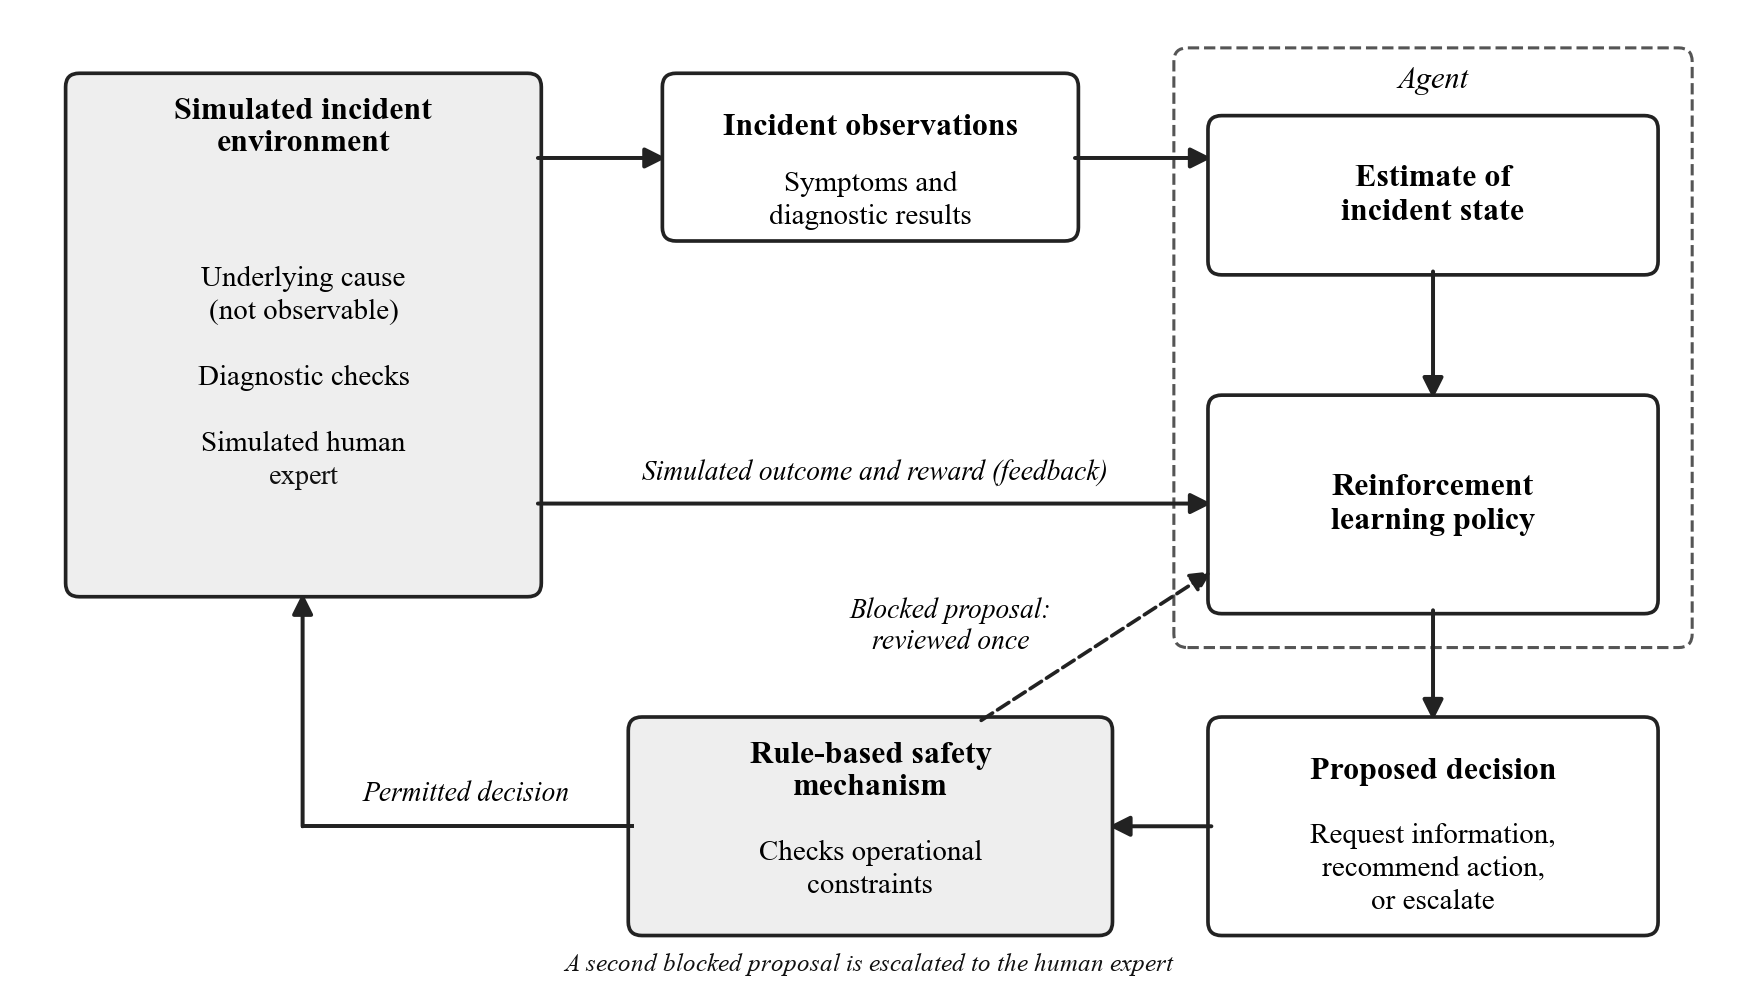
\includegraphics[width=\textwidth]{Figure_1_1_Conceptual_Framework.png}
\caption{Proposed Architecture}
\label{fig:framework}
\end{figure}

\section{The Reinforcement Learning Agents}
\label{sec:agent}

Two learning algorithms are used: a deep Q-network as the primary learner and proximal policy optimisation as a secondary learner, to show whether the findings depend on the choice of algorithm. Both are taken from an established open-source library to limit implementation error~\cite{raffin2021}. Both use action masking: at step $t$ the agent may only choose from the available actions
\begin{equation}
\mathcal{A}_t = \mathcal{A} \setminus \big( \{ a^{\text{chk}}_j : q_{t,j} = 1 \} \cup \mathcal{B}_t \big),
\label{eq:mask}
\end{equation}
which exclude checks already requested and the set $\mathcal{B}_t$ of proposals blocked at this step.

\subsection{Deep Q-Network:}

The deep Q-network (DQN) estimates the action-value function, the expected discounted return of taking action $a$ after observation $o$ and following policy $\pi$ afterwards~\cite{mnih2015}:
\begin{equation}
Q^{\pi}(o, a) = \mathbb{E}_{\pi}\!\left[ \sum_{t' \ge t} \gamma^{t'-t} r_{t'} \;\middle|\; o_t = o,\; a_t = a \right].
\end{equation}
The optimal action values satisfy the Bellman optimality equation, here with the maximum taken only over available actions:
\begin{equation}
Q^{*}(o, a) = \mathbb{E}\!\left[ r_t + \gamma \max_{a' \in \mathcal{A}_{t+1}} Q^{*}(o_{t+1}, a') \;\middle|\; o_t = o,\; a_t = a \right].
\end{equation}

\textbf{Network.} $Q^{*}$ is approximated by a feed-forward neural network with weights $\mathbf{w}$, which takes the encoded observation $\phi(o) \in \mathbb{R}^{n}$ and returns one value for each of the 36 actions. It has two hidden layers of 128 units with rectified linear (ReLU) activations, $\text{ReLU}(v) = \max(0, v)$:
\begin{align}
\mathbf{h}_1 &= \text{ReLU}\big(\mathbf{W}_1 \phi(o) + \mathbf{b}_1\big), & \mathbf{W}_1 &\in \mathbb{R}^{128 \times n}, \\
\mathbf{h}_2 &= \text{ReLU}\big(\mathbf{W}_2 \mathbf{h}_1 + \mathbf{b}_2\big), & \mathbf{W}_2 &\in \mathbb{R}^{128 \times 128}, \\
Q(o, \cdot\,; \mathbf{w}) &= \mathbf{W}_3 \mathbf{h}_2 + \mathbf{b}_3, & \mathbf{W}_3 &\in \mathbb{R}^{|\mathcal{A}| \times 128},
\end{align}
where $\mathbf{w} = \{\mathbf{W}_1, \mathbf{b}_1, \mathbf{W}_2, \mathbf{b}_2, \mathbf{W}_3, \mathbf{b}_3\}$. A tabular method is ruled out because the check states alone admit $4^{20}$ combinations, and the network's output gives a value for every action, so the values the agent assigns to a blocked fix and to escalation can be inspected.

\textbf{Choosing actions.} During training the agent follows an $\epsilon$-greedy policy over the available actions: with probability $1 - \epsilon$ it proposes
\begin{equation}
a_t = \arg\max_{a \in \mathcal{A}_t} Q(o_t, a; \mathbf{w}),
\end{equation}
and with probability $\epsilon$ it proposes an available action chosen uniformly at random. The exploration rate $\epsilon$ decreases during training, and at evaluation $\epsilon = 0$.

\textbf{Learning.} Each transition $(o_t, a_t, r_t, o_{t+1})$ is stored in a replay buffer $\mathcal{E}$, from which mini-batches are sampled. The learning target uses a separate target network with weights $\mathbf{w}^{-}$, copied from $\mathbf{w}$ at fixed intervals, and is masked in the same way as action choice:
\begin{equation}
\tau_t = \begin{cases}
r_t & \text{if } o_{t+1} \text{ is terminal}, \\
r_t + \gamma \max_{a' \in \mathcal{A}_{t+1}} Q(o_{t+1}, a'; \mathbf{w}^{-}) & \text{otherwise}.
\end{cases}
\end{equation}
The weights are updated by gradient descent on the loss
\begin{equation}
\mathcal{L}(\mathbf{w}) = \mathbb{E}_{(o_t, a_t, r_t, o_{t+1}) \sim \mathcal{E}} \Big[ \big( \tau_t - Q(o_t, a_t; \mathbf{w}) \big)^{2} \Big],
\label{eq:dqnloss}
\end{equation}
for which the library uses the Huber form, which is quadratic for small errors and linear for large ones and so limits the effect of outlying targets. The full training loop, with the safety mechanism, is given as Algorithm~\ref{alg:dqn}.

\subsection{Proximal Policy Optimisation:}

Proximal policy optimisation (PPO) learns the policy directly rather than through action values~\cite{schulman2017}. It uses a policy network with weights $\boldsymbol{\vartheta}$ and a value network with weights $\boldsymbol{\psi}$, each with the same two hidden layers of 128 units as the DQN. The policy network outputs a score $f_a(o)$ for each action, and invalid actions are masked by giving them zero probability~\cite{huang2022}:
\begin{equation}
\pi_{\boldsymbol{\vartheta}}(a \mid o_t) = \frac{\exp f_a(o_t)}{\sum_{a' \in \mathcal{A}_t} \exp f_{a'}(o_t)} \quad \text{for } a \in \mathcal{A}_t, \qquad \pi_{\boldsymbol{\vartheta}}(a \mid o_t) = 0 \text{ otherwise}.
\end{equation}
The value network $V_{\boldsymbol{\psi}}(o)$ estimates the expected return from $o$. How much better an action was than expected is measured by the advantage, estimated with generalised advantage estimation~\cite{schulman2016}:
\begin{equation}
\delta_t = r_t + \gamma V_{\boldsymbol{\psi}}(o_{t+1}) - V_{\boldsymbol{\psi}}(o_t), \qquad
\hat{A}_t = \sum_{l=0}^{T-t-1} (\gamma \lambda_{\text{GAE}})^{l}\, \delta_{t+l},
\end{equation}
where $\lambda_{\text{GAE}} \in [0, 1]$ trades bias against variance. PPO limits how far one update can move the policy by clipping the probability ratio between the new and the old policy:
\begin{equation}
\kappa_t(\boldsymbol{\vartheta}) = \frac{\pi_{\boldsymbol{\vartheta}}(a_t \mid o_t)}{\pi_{\boldsymbol{\vartheta}_{\text{old}}}(a_t \mid o_t)}, \qquad
\mathcal{L}^{\text{CLIP}}(\boldsymbol{\vartheta}) = \mathbb{E}_t\Big[ \min\big( \kappa_t \hat{A}_t,\; \text{clip}(\kappa_t, 1 - \epsilon_{\text{clip}}, 1 + \epsilon_{\text{clip}})\, \hat{A}_t \big) \Big].
\end{equation}
The two networks are trained together by maximising
\begin{equation}
\mathcal{L}(\boldsymbol{\vartheta}, \boldsymbol{\psi}) = \mathcal{L}^{\text{CLIP}}(\boldsymbol{\vartheta}) - \nu_1\, \mathbb{E}_t\Big[ \big( V_{\boldsymbol{\psi}}(o_t) - \hat{G}_t \big)^{2} \Big] + \nu_2\, \mathbb{E}_t\Big[ \mathcal{H}\big(\pi_{\boldsymbol{\vartheta}}(\cdot \mid o_t)\big) \Big],
\end{equation}
where $\hat{G}_t = \hat{A}_t + V_{\boldsymbol{\psi}}(o_t)$ is the target return, $\mathcal{H}$ is the entropy of the policy, which encourages exploration, and $\nu_1$ and $\nu_2$ are weighting coefficients.

\subsection{Training:}

Training begins from the library's default hyperparameters, and a small search over the learning rate, the network size and the exploration schedule is carried out on seeds that are not used in the final experiments. The training length is set in pilot runs as the point at which the mean return stops improving. Each agent will be trained with ten random seeds in two regimes: at the base ambiguity level $\ell_0$, and with $\ell$ drawn at random from its planned ranges at the start of each episode. Comparing the two regimes shows whether robustness requires exposure to ambiguity during training. Table~\ref{tab:agentsymbols} summarises the symbols introduced for the agents.

{\small
\begin{longtable}{|P{2.8cm}|P{12.2cm}|}
\caption{Symbols used for the problem, the environment and the agents}
\label{tab:agentsymbols} \\
\hline
\textbf{Symbol} & \textbf{Meaning} \\ \hline
\endfirsthead
\hline
\textbf{Symbol} & \textbf{Meaning} \\ \hline
\endhead
\multicolumn{2}{r}{\emph{Continued on next page}} \\
\endfoot
\endlastfoot
\multicolumn{2}{|l|}{\textit{Problem and environment}} \\ \hline
$\mathcal{C}$, $c_m$, $K$ & Set of causes, the $m$-th cause, number of causes \\ \hline
$c$ & The hidden true cause of the current incident \\ \hline
$\mathcal{D}$, $d_j$, $J$, $k_j$ & Set of diagnostic checks, the $j$-th check, number of checks, cost of check $d_j$ \\ \hline
$\mathcal{X}$, $x$ & Set of incident contexts, the context of the current incident \\ \hline
$\theta_{jm}$ & Probability that check $d_j$ is positive when the cause is $c_m$ \\ \hline
$\sigma_e$, $E$, $\varphi_{em}$ & The $e$-th symptom (1 if present); number of symptoms; probability that symptom $e$ is present when the cause is $c_m$ \\ \hline
$s_t$, $\mathbf{z}$, $\mathbf{q}_t$ & State at step $t$; vector of check results; vector of checks requested by step $t$ \\ \hline
$\mathcal{A}$, $a_t$ & Set of actions; action proposed at step $t$ \\ \hline
$a^{\text{chk}}_j$, $a^{\text{fix}}_m$, $a_{\text{esc}}$ & Request check $d_j$; recommend the fix for cause $c_m$; escalate \\ \hline
$o_t$, $\mathbf{u}_t$, $\boldsymbol{\sigma}$, $\beta_t$ & Observation at step $t$; check states; symptoms; blocked flag \\ \hline
$\phi(o_t)$, $n$ & Encoded observation vector and its length \\ \hline
$r_t$, $r_{\text{correct}}$, $\lambda_{\text{wrong}}$, $\lambda_{\text{esc}}$, $\lambda_{\text{block}}$ & Reward at step $t$; reward for a correct fix; penalty for a wrong fix; cost of an escalation; penalty for a blocked proposal \\ \hline
$\gamma$, $H$, $T$ & Discount factor; step limit; length of an episode \\ \hline
$b_t(c_m)$, $\mathcal{I}_t$ & Belief that the cause is $c_m$ at step $t$; checks whose results have been observed by step $t$ \\ \hline
$\rho_q$, $N_\rho$ & The $q$-th operational rule; number of rules \\ \hline
$\mathcal{A}_{\text{safe}}$ & Actions permitted by all the rules \\ \hline
$a^{(1)}_t$, $a^{(2)}_t$, $a^{\text{exec}}_t$ & First proposal, second proposal and action carried out at step $t$ \\ \hline
$\mathcal{A}_t$, $\mathcal{B}_t$ & Available actions at step $t$; proposals blocked at step $t$ \\ \hline
$\eta(\pi)$ & Expected discounted return of policy $\pi$ \\ \hline
$p_{\text{miss}}$, $p_{\text{noise}}$, $\omega$ & Probabilities that a check is missing or reversed; overlap between causes in a category \\ \hline
$\tilde{\theta}_{jm}$, $\theta'_{jm}$, $\varphi'_{em}$, $g(m)$ & Check likelihood after noise; check and symptom likelihoods after overlap; category of cause $c_m$ \\ \hline
$y$ & Reference label: 1 if the incident should be escalated \\ \hline
\multicolumn{2}{|l|}{\textit{Deep Q-network}} \\ \hline
$Q^{\pi}(o,a)$, $Q^{*}$ & Action value under policy $\pi$; optimal action value \\ \hline
$\mathbf{w}$, $\mathbf{w}^{-}$ & Weights of the Q-network and of the target network \\ \hline
$\mathbf{W}_\cdot$, $\mathbf{b}_\cdot$, $\mathbf{h}_\cdot$ & Weight matrices, bias vectors and hidden-layer outputs \\ \hline
$\epsilon$ & Exploration rate of the $\epsilon$-greedy policy \\ \hline
$\mathcal{E}$, $\tau_t$, $\mathcal{L}$ & Replay buffer; learning target; loss \\ \hline
\multicolumn{2}{|l|}{\textit{Proximal policy optimisation}} \\ \hline
$\boldsymbol{\vartheta}$, $\boldsymbol{\psi}$ & Weights of the policy network and of the value network \\ \hline
$f_a(o)$, $\pi_{\boldsymbol{\vartheta}}$, $V_{\boldsymbol{\psi}}$ & Score of action $a$; policy; value estimate \\ \hline
$\delta_t$, $\hat{A}_t$, $\lambda_{\text{GAE}}$ & Temporal-difference error; estimated advantage; advantage-estimation parameter \\ \hline
$\kappa_t$, $\epsilon_{\text{clip}}$ & Probability ratio between new and old policy; clipping range \\ \hline
$\hat{G}_t$, $\mathcal{H}$, $\nu_1$, $\nu_2$ & Target return; policy entropy; loss weights \\ \hline
\end{longtable}
}

\section{Baseline Decision Policies}
\label{sec:baselines}

The agent will be compared with six baseline policies that run in the same environment on the same evaluation incidents, each standing for an approach from Chapter~2 (Table~\ref{tab:baselines}).

\begin{table}[H]
\centering
\caption{Baseline decision policies}
\label{tab:baselines}
\small
\begin{tabular}{|p{3.4cm}|p{7.4cm}|p{4.2cm}|}
\hline
\textbf{Policy} & \textbf{Behaviour} & \textbf{Approach represented} \\ \hline
Initial-symptom & Recommends the fix for the cause that the prior and the symptoms make most likely (Equation~\eqref{eq:belief} at $t = 0$), without checks & Triage as one prediction \\ \hline
Scripted checklist & Requests a fixed sequence of checks for the category, elicited from Directorate practice, then recommends & Runbook practice \\ \hline
Always-escalate & Escalates every incident & The limit of deferral \\ \hline
Confidence threshold & Tracks the belief $b_t$ of Equation~\eqref{eq:belief}, requests the most informative check until one cause passes a threshold, else escalates & Uncertainty-driven investigation (knows the model) \\ \hline
Unconstrained agent & The same DQN without the safety mechanism & Standard shielding comparison \\ \hline
Penalty-only agent & The same DQN without the mechanism, with a reward penalty per rule violation & Constraint by reward penalty \\ \hline
\end{tabular}
\end{table}

The confidence-threshold policy is given as Algorithm~\ref{alg:threshold}. Two ablations of the agent, one that cannot request checks and one that cannot escalate, will show what each option contributes.

\section{Evaluation Strategy}
\label{sec:evaluation}

The framework will be evaluated across four groups of measures: decision quality, investigation efficiency, escalation behaviour and constraint compliance. At each level of ambiguity, $S = 10$ evaluation sets of $N = 1{,}000$ incidents each are generated from seeds never used in training, and every policy is run on the same sets. Set $s$ is paired with training seed $s$ of each learning agent; a baseline that does not learn is run on all $S$ sets, so that every policy has $S$ values of each measure. With $N = 1{,}000$, the standard error of a rate measured on one set is at most $\sqrt{0.25/1000} \approx 0.016$, small enough to resolve the differences of 0.05 used in the decision criteria (Section~\ref{sec:criteria}). Each episode $i$ ends in one of three outcomes $o_i$: a correct recommendation (c), a wrong recommendation (w) or an escalation (e). Let $N_{\text{c}}$, $N_{\text{w}}$ and $N_{\text{e}}$ be the numbers of episodes with each outcome, so that
\begin{equation}
N = N_{\text{c}} + N_{\text{w}} + N_{\text{e}}.
\end{equation}
Escalations include those chosen by the agent, those forced by the safety mechanism and those caused by the step limit. Table~\ref{tab:notation} defines the symbols used in the rest of this section.

{\small
\begin{longtable}{|P{2.6cm}|P{12.4cm}|}
\caption{Symbols used in the evaluation measures}
\label{tab:notation} \\
\hline
\textbf{Symbol} & \textbf{Meaning} \\ \hline
\endfirsthead
\hline
\textbf{Symbol} & \textbf{Meaning} \\ \hline
\endhead
\multicolumn{2}{r}{\emph{Continued on next page}} \\
\endfoot
\endlastfoot
\multicolumn{2}{|l|}{\textit{Episodes and outcomes}} \\ \hline
$N$ & Number of incidents in one evaluation set ($N = 1{,}000$); each episode is the triage of one incident \\ \hline
$i$ & Index of an evaluation episode, $i = 1, \dots, N$ \\ \hline
$o_i$ & Outcome of episode $i$: c (correct recommendation), w (wrong recommendation) or e (escalation) \\ \hline
$N_{\text{c}}, N_{\text{w}}, N_{\text{e}}$ & Numbers of episodes ending in a correct recommendation, a wrong recommendation and an escalation \\ \hline
$T_i$ & Number of steps taken in episode $i$ \\ \hline
$r_{i,t}$ & Reward received at step $t$ of episode $i$ \\ \hline
$\pi$ & A decision policy: the proposed agent or one of the baselines \\ \hline
\multicolumn{2}{|l|}{\textit{Investigation}} \\ \hline
$K_i$ & Set of diagnostic checks requested in episode $i$; $|K_i|$ is their number \\ \hline
$k_j$ & Cost of diagnostic check $j$ \\ \hline
\multicolumn{2}{|l|}{\textit{Escalation}} \\ \hline
$y_i$ & Reference label of episode $i$: 1 if the incident should be escalated, 0 otherwise \\ \hline
$\hat{y}_i$ & Agent's choice in episode $i$: 1 if it chose to escalate, 0 otherwise \\ \hline
TP, FP, FN, TN & True positives, false positives, false negatives and true negatives: the four cells of the confusion matrix of $\hat{y}_i$ against $y_i$ \\ \hline
\multicolumn{2}{|l|}{\textit{Constraint compliance}} \\ \hline
$M$ & Total number of actions proposed by the agent over the evaluation episodes \\ \hline
$M_{\text{b}}$ & Number of proposed actions blocked by the safety mechanism \\ \hline
$N_{\text{f}}$ & Number of episodes ending in a forced escalation after a second blocked proposal \\ \hline
$N_{\text{v}}$ & Number of episodes in which a prohibited action took effect \\ \hline
$v_i$ & 1 if a prohibited action took effect in episode $i$, 0 otherwise \\ \hline
$\mathbf{1}[\cdot]$ & Indicator function: 1 when the condition in brackets holds, 0 otherwise \\ \hline
\multicolumn{2}{|l|}{\textit{Robustness and reporting}} \\ \hline
$\ell$ & Level of ambiguity, set by $p_{\text{miss}}$, $p_{\text{noise}}$ and $\omega$ (Section~\ref{sec:environment}) \\ \hline
$\ell_0$ & Base level of ambiguity, at which the agent is trained in the first regime \\ \hline
$S$ & Number of training seeds per learning agent, and of evaluation sets per ambiguity level ($S = 10$) \\ \hline
$s$ & Index of a seed, $s = 1, \dots, S$ \\ \hline
$X$, $X_s$, $\bar{X}$ & Any measure; its value on seed $s$; its mean over seeds \\ \hline
$B$ & Number of bootstrap resamples used for the confidence interval ($B = 10{,}000$) \\ \hline
\multicolumn{2}{|l|}{\textit{Measures}} \\ \hline
Acc & Resolution accuracy \\ \hline
Cov & Coverage: share of incidents on which the agent makes a recommendation \\ \hline
SelAcc & Selective accuracy: accuracy of the recommendations made \\ \hline
WR & Wrong-recommendation rate \\ \hline
$\bar{G}$ & Mean episodic return \\ \hline
$\bar{n}$, $\bar{C}$ & Mean number of checks and mean investigation cost per episode \\ \hline
ER & Escalation rate \\ \hline
$P$, $R$, $F_1$ & Escalation precision, recall and F1 score \\ \hline
MCC & Matthews correlation coefficient of escalations \\ \hline
PVR & Proposed-violation rate \\ \hline
FER & Forced-escalation rate \\ \hline
EVR & Executed-violation rate \\ \hline
CSR & Compliant success rate \\ \hline
$\Delta\text{Acc}(\ell)$ & Change in resolution accuracy at level $\ell$ relative to $\ell_0$ \\ \hline
$\mathbf{m}(\ell)$ & Decision mix at level $\ell$: coverage, escalation rate and mean number of checks \\ \hline
\end{longtable}
}

\subsection{Decision Quality:}

Decision quality describes how often the final decision is right. Resolution accuracy is the share of all incidents that the agent resolves itself, the usual accuracy of the triage literature~\cite{remil2024}:
\begin{equation}
\text{Acc} = \frac{N_{\text{c}}}{N}.
\end{equation}
Because an agent can avoid errors by escalating, accuracy is read together with coverage and selective accuracy, the standard pair of selective prediction~\cite{geifman2019}:
\begin{equation}
\text{Cov} = \frac{N_{\text{c}} + N_{\text{w}}}{N}, \qquad
\text{SelAcc} = \frac{N_{\text{c}}}{N_{\text{c}} + N_{\text{w}}}.
\end{equation}
The wrong-recommendation rate isolates the most costly error in triage:
\begin{equation}
\text{WR} = \frac{N_{\text{w}}}{N}.
\end{equation}
The mean episodic return is the quantity the agent is trained to maximise~\cite{sutton2018}:
\begin{equation}
\bar{G} = \frac{1}{N}\sum_{i=1}^{N}\sum_{t=0}^{T_i-1} r_{i,t},
\end{equation}
where $T_i$ is the number of steps in episode $i$ and $r_{i,t}$ is the reward at step $t$. Because $\bar{G}$ depends on the reward values chosen, it is never reported alone.

\subsection{Investigation Efficiency:}

Investigation efficiency describes what the agent spends on evidence before it decides. Let $K_i$ be the set of checks requested in episode $i$ and $k_j$ the cost of check $j$. The mean number of checks and the mean investigation cost are
\begin{equation}
\bar{n} = \frac{1}{N}\sum_{i=1}^{N} |K_i|, \qquad
\bar{C} = \frac{1}{N}\sum_{i=1}^{N}\sum_{j \in K_i} k_j.
\end{equation}
The cost stands in for time, which a simulation without a clock cannot measure directly. Following the evaluation of costly feature acquisition~\cite{janisch2019}, each policy $\pi$ is also plotted as a point $(\bar{C}_\pi, \text{Acc}_\pi)$ on an accuracy--cost curve, which shows whether additional investigation buys additional accuracy and allows policies to be compared at equal cost.

\subsection{Escalation Behaviour:}

Escalation behaviour describes how much the agent hands to the human expert and whether it hands over the right cases. The escalation rate is the load placed on human experts~\cite{turan2026}:
\begin{equation}
\text{ER} = \frac{N_{\text{e}}}{N}.
\end{equation}
The remaining measures compare the agent's own choices with the reference labels. For each episode, let $y_i = 1$ if the incident is labelled as one that should be escalated and $y_i = 0$ otherwise, and let $\hat{y}_i = 1$ if the agent chose to escalate and $\hat{y}_i = 0$ otherwise. Forced escalations and step-limit escalations are excluded, because the agent did not choose them; they are reported under constraint compliance. Over the remaining episodes,
\begin{equation}
\text{TP} = \sum_i \hat{y}_i\, y_i, \quad
\text{FP} = \sum_i \hat{y}_i (1-y_i), \quad
\text{FN} = \sum_i (1-\hat{y}_i)\, y_i, \quad
\text{TN} = \sum_i (1-\hat{y}_i)(1-y_i).
\end{equation}
Escalation precision is the share of the agent's escalations that should have been escalated; low precision means that human experts receive incidents the agent could have resolved. Escalation recall is the share of incidents that should have been escalated that the agent did escalate; low recall means the agent kept incidents it should have handed over. The F1 score is their harmonic mean:
\begin{equation}
P = \frac{\text{TP}}{\text{TP}+\text{FP}}, \qquad
R = \frac{\text{TP}}{\text{TP}+\text{FN}}, \qquad
F_1 = \frac{2PR}{P+R}.
\end{equation}
Because precision, recall and F1 can all look acceptable when one class is rare, the Matthews correlation coefficient, which uses all four cells of the confusion matrix and exposed degenerate triage policies that F1 concealed~\cite{okafor2026}, is also reported:
\begin{equation}
\text{MCC} = \frac{\text{TP}\cdot\text{TN} - \text{FP}\cdot\text{FN}}
{\sqrt{(\text{TP}+\text{FP})(\text{TP}+\text{FN})(\text{TN}+\text{FP})(\text{TN}+\text{FN})}}.
\end{equation}
MCC ranges from $-1$ to $+1$, where $0$ means the agent's escalations are no better than chance.

\subsection{Constraint Compliance:}

Constraint compliance describes the agent's relationship to the rules. Let $M$ be the total number of actions the agent proposes over the evaluation episodes and $M_{\text{b}}$ the number blocked by the safety mechanism. The proposed-violation rate shows whether the agent has learned to act within the rules or relies on being stopped:
\begin{equation}
\text{PVR} = \frac{M_{\text{b}}}{M}.
\end{equation}
Let $N_{\text{f}}$ be the number of episodes that end in a forced escalation after a second blocked proposal, and $N_{\text{v}}$ the number in which a prohibited action takes effect. The forced-escalation rate and the executed-violation rate are
\begin{equation}
\text{FER} = \frac{N_{\text{f}}}{N}, \qquad
\text{EVR} = \frac{N_{\text{v}}}{N}.
\end{equation}
The executed-violation rate is zero by construction when the mechanism is active, and it is the central measure for the unconstrained and penalty-only agents, as in the shielding literature~\cite{alshiekh2018}. Let $v_i = 1$ if a prohibited action took effect in episode $i$. The compliant success rate, which follows the measure of task completion under policy used for agent benchmarks~\cite{levy2026}, is
\begin{equation}
\text{CSR} = \frac{1}{N}\sum_{i=1}^{N} \mathbf{1}\left[o_i = \text{c} \;\wedge\; v_i = 0\right],
\end{equation}
where $\mathbf{1}[\cdot]$ equals 1 when its condition holds and 0 otherwise. For agents without the mechanism, the gap between Acc and CSR shows how much of their accuracy was obtained by breaking rules.

\subsection{Robustness:}

Robustness is not a separate metric: every measure above is computed at each ambiguity level $\ell$ and reported as a function of it. Degradation is the change relative to the base level $\ell_0$, for example
\begin{equation}
\Delta\text{Acc}(\ell) = \text{Acc}(\ell) - \text{Acc}(\ell_0),
\end{equation}
and likewise for the wrong-recommendation rate. The decision mix at each level,
\begin{equation}
\mathbf{m}(\ell) = \big(\text{Cov}(\ell),\; \text{ER}(\ell),\; \bar{n}(\ell)\big),
\end{equation}
shows whether the agent responds to ambiguity by investigating more, by escalating more, or by continuing to recommend on weaker evidence, which is the behaviour tested by hypotheses H3a to H3c.

\subsection{Reporting:}

Each learning agent is trained with $S = 10$ random seeds, and each seed is evaluated on its paired evaluation set. For any measure $X$, the reported value is the mean over the $S$ values,
\begin{equation}
\bar{X} = \frac{1}{S}\sum_{s=1}^{S} X_s,
\end{equation}
with a 95\% percentile bootstrap confidence interval obtained by resampling the $S$ values with replacement $B = 10{,}000$ times and taking the 2.5th and 97.5th percentiles of the resampled means~\cite{agarwal2021}.

\subsection{Decision Criteria:}
\label{sec:criteria}

The hypotheses are judged by the following criteria, fixed before any experiment is run. A policy is said to score \emph{higher} than another on a rate when its mean exceeds the other's by at least 0.05 and the two 95\% bootstrap confidence intervals do not overlap; \emph{lower} is defined in the same way. For the mean number of checks, the minimum difference is 0.5 checks. Any other outcome counts as no difference.
\begin{itemize}
\item \textbf{H1} is supported if, at $\ell_0$, the agent's resolution accuracy is higher than that of each of the initial-symptom, scripted-checklist and always-escalate policies, and its mean investigation cost is not higher than that of the scripted checklist. Otherwise it is not supported.
\item \textbf{H2} is supported if, at $\ell_0$, the agent's compliant success rate is higher than that of both the unconstrained agent and the penalty-only agent. The executed-violation rate of the agent with the mechanism is checked separately as a verification of the implementation: it must be zero on every evaluation incident, and any other value is treated as a defect to be corrected before results are reported.
\item \textbf{H3a to H3c} are judged one factor at a time, by comparing the agent at $\ell_0$ with the agent at the highest planned value of the factor concerned, the other two factors held at their base values. H3a is supported if, as $p_{\text{miss}}$ rises, the escalation rate is higher and the mean number of checks is not higher. H3b is supported if, as $p_{\text{noise}}$ rises, the mean number of checks is higher and coverage is lower. H3c is supported if, as $\omega$ rises, the mean number of checks and the escalation rate are both higher.
\end{itemize}
Each hypothesis is reported as supported or not supported, whichever the results show.

\subsection{Experiments:}

Four experiments use these measures. Experiment~1 compares the agent with the six baselines at the base level of ambiguity, and is repeated with the PPO agent to check that the findings do not depend on the learning algorithm. Experiment~2 compares the agent with the unconstrained and penalty-only agents and tracks the proposed-violation rate over training. Experiment~3 compares it with its two ablations. Experiment~4 evaluates every policy across ambiguity levels, for both training regimes. Its sweep is one factor at a time from $\ell_0$: each control takes its three non-base planned values while the other two stay at their base values, giving nine levels, which with $\ell_0$ make ten. Two combined levels are added, with all three controls at their second-highest and at their highest planned values, giving twelve ambiguity settings in all. A sensitivity analysis repeats Experiment~1 with the escalation cost set to $\lambda_{\text{esc}} \in \{1, 3, 6, 9\}$, all below $\lambda_{\text{wrong}}$. All measures are computed on the evaluation sets described at the start of this section, following Algorithm~\ref{alg:evaluation}.

\section{Limitations}
\label{sec:limitations}

The design has limitations that bound what its results can show.
\begin{itemize}[nosep]
\item \textbf{Simulation and reality.} The agent is trained and evaluated only in a simulator built from staff ratings, so the results show how it behaves in that model, not how it would perform at the Directorate.
\item \textbf{An expert who always succeeds.} The simulated human expert resolves every escalated incident, so escalation is never itself a source of error, and its only cost is $\lambda_{\text{esc}}$.
\item \textbf{A low cost of escalation.} With $\lambda_{\text{esc}} = 3$ against $\lambda_{\text{wrong}} = 10$, escalation is cheap relative to a wrong fix, which may understate its burden on experts and encourage escalation; the sensitivity analysis over $\lambda_{\text{esc}} \in \{1, 3, 6, 9\}$ shows how far the conclusions depend on this value.
\item \textbf{Conditional independence.} Symptoms and check results are assumed to be independent given the cause. In practice, checks that read the same logs may be correlated, which would make evidence less informative than the simulator assumes.
\item \textbf{Researcher-chosen rewards.} The reward values are set by the researcher and tuned in pilot runs, not measured at the Directorate, and the agent's behaviour depends on them.
\item \textbf{One institution.} The scenario model comes from a single IT directorate, so its causes, checks, rules and ratings may not represent other organisations.
\end{itemize}


\chapter{Expected Results}
\label{ch:chapter-04}
\section{Decision Quality}

The agent is expected to achieve higher decision quality than the selected baseline policies in ambiguous incident scenarios (hypothesis H1). Specifically, it is expected to resolve a larger share of incidents correctly than the initial-symptom, scripted and always-escalate policies at equal or lower investigation cost, and to approach the confidence-threshold policy without being given the likelihood model. Numerical targets will be fixed after the pilot runs, and the results will be reported whether or not the hypothesis holds.

\section{Rule Compliance}

With the safety mechanism in place, the agent is expected to achieve a higher rate of rule-compliant correct recommendations than the same agent without it (hypothesis H2). No prohibited action will be executed when the mechanism is active, so the comparison of interest is the compliant success rate against the unconstrained and penalty-only agents. The proposed-violation rate is expected to fall over training, which would show that the agent learns to act within the rules and does not rely on being stopped.

\section{Robustness to Ambiguity}

As the level of ambiguity rises, the agent is expected to request more diagnostic information and to escalate more incidents, and not to continue recommending fixes on weaker evidence (hypothesis H3). The agent trained across randomised ambiguity levels is expected to degrade less than the agent trained at a single level. The experiments will report what no reviewed study has reported: how the shares of investigating, recommending and escalating change across controlled levels of missing, unreliable and overlapping evidence.

\section{Prototype}

The research is expected to produce a working simulator of IT incident triage built from the Directorate's scenarios, the rule-based safety mechanism, six baseline policies, trained agents, and scripts that reproduce every experiment. A lightweight dashboard will replay an incident step by step, showing the evidence revealed, the agent's estimated action values, any blocked proposal and the final decision, beside the comparison results.

\textbf{Broader impact.} Putting this together, the expected results address the problem this research is concerned with: that automated triage tools predict an answer for every incident and do not know when to look further, when to act within the rules, and when to hand the incident to a person. An agent that makes these three decisions under explicit, readable rules, evaluated on all four groups of measures, would give IT support teams such as the Directorate evidence on how far such automation can be trusted before it is considered for use.


%%%=== =============Add bibliography & references
\bibliographystyle{IEEEtran}
\bibliography{../thesis/citations/references,proposal_extra}
\addcontentsline{toc}{chapter}{REFERENCES}


%%%==== Add Appendicies ==

\appendix
\addcontentsline{toc}{chapter}{APPENDICIES}
\begin{appendices}
    
%----- Budget ---
\chapter{Budget  }
\label{App:budget}
The research has few direct costs. Training and evaluation will run on the university's computing facilities and the researcher's laptop with open-source software (Python, Gymnasium, Stable-Baselines3 and PyTorch), and the elicitation sessions with the Directorate of University ICT Services involve no cost. The only expected cost is printing. Unit costs are estimates based on the author's earlier proposal budget.

\begin{longtable}{|c|P{4.2cm}|P{4.2cm}|>{\raggedleft\arraybackslash}p{2.0cm}|c|>{\raggedleft\arraybackslash}p{2.0cm}|}
\hline
\textbf{No.} & \textbf{Item} & \textbf{Details} & \textbf{Unit Cost (UGX)} & \textbf{Qty} & \textbf{Total (UGX)} \\ \hline
1 & Project report printing and binding & 3 copies for the supervisor, department, personal & 50,000 & 3 & 150,000 \\ \hline
2 & Proposal printing & 2 copies for supervisor review & 10,000 & 2 & 20,000 \\ \hline
\multicolumn{5}{|r|}{\textbf{TOTAL BUDGET (UGX)}} & \textbf{170,000} \\ \hline
\end{longtable}



\chapter{Research Project timelines }
\label{App:research-project-timelines}
The project is managed in seven phases. The implementation runs over six weeks, from 19 October to 29 November 2026, after the literature review and the stakeholder interview. Each phase depends on the one before it: the environment cannot be built before the scenarios are elicited, the scenario model is frozen before any agent is trained, and the experiments cannot run before the agents and baselines exist.

The seven phases group the eight research phases of Figure~\ref{fig:pipeline} for scheduling. Phase~1 covers specifying the problem; Phase~2, eliciting scenarios with the Directorate; Phase~3, both building and validating the environment and encoding the rules; Phase~4, both implementing the baselines and training the agents; Phase~5, running the experiments; and Phase~6, analysing the results. Phase~7, writing and submission, is not a research phase and so does not appear in Figure~\ref{fig:pipeline}.

\begin{center}\textbf{Project Timeline (19 October to 29 November 2026)}\end{center}

{\small
\begin{longtable}{|c|P{2.3cm}|P{4.8cm}|P{1.5cm}|P{1.6cm}|P{3.0cm}|}
\hline
\textbf{Phase} & \textbf{Phase Name} & \textbf{Key Activities} & \textbf{Weeks} & \textbf{Depends on} & \textbf{Deliverable} \\ \hline
\endfirsthead
\hline
\textbf{Phase} & \textbf{Phase Name} & \textbf{Key Activities} & \textbf{Weeks} & \textbf{Depends on} & \textbf{Deliverable} \\ \hline
\endhead
\multicolumn{6}{r}{\emph{Continued on next page}} \\
\endfoot
\endlastfoot
1 & Literature and Planning & Thematic literature review and Chapters 1--3; stakeholder interview with the Directorate (19 Oct); systematic literature review (23 Oct); approvals; elicitation workbook. & Before 19 Oct, Week 1 & -- & Proposal, systematic review, elicitation workbook. \\ \hline
2 & Scenario Elicitation & Elicitation session(s) with Directorate staff in the week of 26 October; scenario model of about 15 causes, about 10 symptoms, 20 checks and 10 rules written up as configuration files. & Week 2 & 1 & Scenario model v1. \\ \hline
3 & Environment and Rules & Incident generator and Gymnasium environment with the three ambiguity controls; the rules and the review-then-escalate mechanism; tests and leakage check; staff review of sample incidents; scenario model frozen at the end of the week. & Week 3 & 2 & Frozen scenario model; tested simulator and rule mechanism. \\ \hline
4 & Baselines and Training & Six baseline policies and the metrics module; pilot runs; small hyperparameter search; the agent, unconstrained and penalty-only agents and the PPO agent trained over ten seeds on the frozen model. & Week 4 & 3 & Baselines run end to end; trained agents. \\ \hline
5 & Experiments & Experiments 1--3 (baselines, effect of the mechanism, ablations); sensitivity to escalation cost; Experiment 4 (twelve ambiguity settings). & Week 5 & 4 & Results tables and charts. \\ \hline
6 & Analysis and Prototype & Confidence intervals, decision-mix charts and findings against the decision criteria for H1--H3; replay dashboard and results panel. & Weeks 5--6 & 5 & Findings summary; working prototype. \\ \hline
7 & Writing and Submission & Results chapter, revision of Chapters 1--3, poster, archive of code and configurations, presentation rehearsal. & Week 6 & 6 & Poster, report, archived code. \\ \hline
\end{longtable}
}

\begin{figure}[H]
\centering
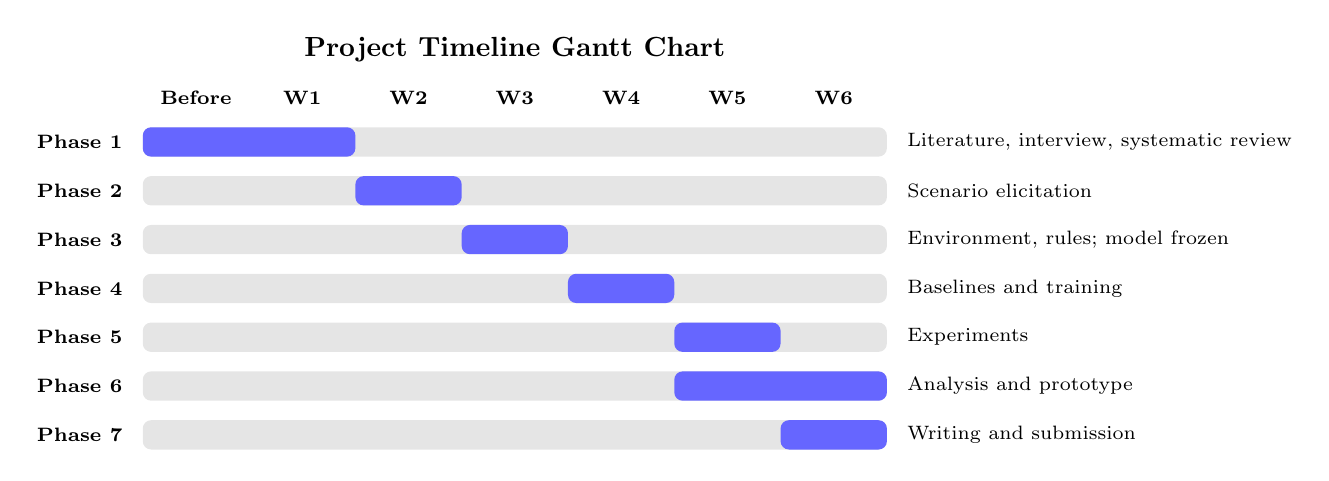
\begin{tikzpicture}[x=1.35cm,y=0.62cm]
\node[font=\bfseries] at (3.5,8.4) {Project Timeline Gantt Chart};
\foreach \w/\lab in {0/{Before},1/{W1},2/{W2},3/{W3},4/{W4},5/{W5},6/{W6}}
  \node[font=\scriptsize\bfseries] at (\w+0.5,7.4) {\lab};
\foreach \r/\lab/\s/\e/\d in {
  7/{Phase 1}/0/2/{Literature, interview, systematic review},
  6/{Phase 2}/2/3/{Scenario elicitation},
  5/{Phase 3}/3/4/{Environment, rules; model frozen},
  4/{Phase 4}/4/5/{Baselines and training},
  3/{Phase 5}/5/6/{Experiments},
  2/{Phase 6}/5/7/{Analysis and prototype},
  1/{Phase 7}/6/7/{Writing and submission}} {
  \node[font=\scriptsize\bfseries,anchor=east] at (-0.1,\r-0.5) {\lab};
  \fill[gray!20,rounded corners=3pt] (0,\r-0.8) rectangle (7,\r-0.2);
  \fill[blue!60,rounded corners=3pt] (\s,\r-0.8) rectangle (\e,\r-0.2);
  \node[font=\scriptsize,anchor=west] at (7.1,\r-0.5) {\d};
}
\end{tikzpicture}
\caption{Research project timeline Gantt chart. W1 begins on 19 October 2026 and W6 ends on 29 November 2026. The scenario model is frozen at the end of W3, before training begins in W4.}
\end{figure}



%-- Declaration of AI Usage
\chapter{Declaration of AI use }
\label{App:AI-use-declaration}
\textbf{Declaration Statement:}

I, \theStudentName, declare that I used

\begin{enumerate}[label=\roman*.]

\item \textit{\textbf{Claude by Anthropic (Claude Opus 5.5)}} as a research assistant and sparring partner throughout the development of this research. I used it to review my arguments, identify weaknesses in my reasoning, and suggest improvements to the clarity and structure of my work. I also used it to assist with the systematic literature review, including refining search strategies, reviewing literature, and strengthening the discussion of research gaps. I evaluated the suggestions and retained or modified them based on my own research and understanding.

\item \textit{\textbf{Claude by Anthropic}} to assist with the technical presentation of my research, including writing and formatting LaTeX code for tables, generating some figures, and improving document layout. I reviewed the generated code and outputs and made the necessary modifications to ensure that they accurately represented my work.

\end{enumerate}


\vspace{1cm}

Signature: \line(1,0){8.0cm}
Date:	\line(1,0){4.0cm}\par



%-- Major publications
\chapter{List of 10 Major Publications Reviewed}
\label{App:major-journal-publications-reviewed}
The publications are listed in order of their relevance to this research: three review papers, four journal articles and three conference papers. \todo{Fill in the impact factors from the Journal Citation Reports or Scopus; they have not been verified.}

\begin{center}\textbf{Publications Ranked by Relevance}\end{center}

{\small
\begin{longtable}{|c|P{5.6cm}|P{3.6cm}|P{2.2cm}|P{1.6cm}|}
\hline
\textbf{Rank} & \textbf{Title} & \textbf{Journal / Venue} & \textbf{Type} & \textbf{Impact Factor} \\ \hline
\endfirsthead
\hline
\textbf{Rank} & \textbf{Title} & \textbf{Journal / Venue} & \textbf{Type} & \textbf{Impact Factor} \\ \hline
\endhead
\multicolumn{5}{r}{\emph{Continued on next page}} \\
\endfoot
\endlastfoot
\rowcolor{green!15} 1 & Sahin \& Mert (2026): Dual-Threshold Conformal Deferral for Trustworthy Security Alert Triage~\cite{sahin2026} & Electronics & Journal Article & \todo{TBC} \\ \hline
\rowcolor{green!15} 2 & Kovtun et al.\ (2026): Risk-Sensitive Decision-Making in SOC Alert Escalation under Resource Constraints~\cite{kovtun2026} & CEUR Workshop Proceedings & Conference Paper & \todo{TBC} \\ \hline
\rowcolor{green!15} 3 & Okafor (2026): A Leakage-Free Benchmark of Offline Policy Learning for SOC Alert Triage~\cite{okafor2026} & Machine Learning with Applications & Journal Article & \todo{TBC} \\ \hline
\rowcolor{green!15} 4 & Hammar et al.\ (2026): Adaptive Network Security Policies via Belief Aggregation and Rollout~\cite{hammar2026belief} & IEEE Transactions on Information Forensics and Security & Journal Article & \todo{TBC} \\ \hline
\rowcolor{green!15} 5 & Chen et al.\ (2020): Towards Intelligent Incident Management~\cite{chen2020} & ESEC/FSE & Conference Paper & \todo{TBC} \\ \hline
\rowcolor{green!15} 6 & Remil et al.\ (2024): AIOps Solutions for Incident Management~\cite{remil2024} & arXiv & Review & \todo{TBC} \\ \hline
\rowcolor{yellow!25} 7 & Alshiekh et al.\ (2018): Safe Reinforcement Learning via Shielding~\cite{alshiekh2018} & AAAI Conference on Artificial Intelligence & Conference Paper & \todo{TBC} \\ \hline
\rowcolor{yellow!25} 8 & K\"{o}nighofer et al.\ (2025): Shields for Safe Reinforcement Learning~\cite{konighofer2025} & Communications of the ACM & Review & \todo{TBC} \\ \hline
\rowcolor{yellow!25} 9 & Garc\'{\i}a \& Fern\'{a}ndez (2015): A Comprehensive Survey on Safe Reinforcement Learning~\cite{garcia2015} & Journal of Machine Learning Research & Review & \todo{TBC} \\ \hline
\rowcolor{yellow!25} 10 & Mnih et al.\ (2015): Human-Level Control through Deep Reinforcement Learning~\cite{mnih2015} & Nature & Journal Article & \todo{TBC} \\ \hline
\end{longtable}
}

\textbf{Relevance Key}

{\small
\begin{tabular}{|p{1cm}|p{12cm}|}
\hline
\cellcolor{green!15} & Addresses reinforcement learning or sequential decisions in IT or security incident handling \\ \hline
\cellcolor{yellow!25} & Provides the methods the study builds on: safe reinforcement learning, shielding, deep Q-networks \\ \hline
\end{tabular}
}



%--------- Search strings used to arrive at the publications
\chapter{Scopus Search Strings used during the literature review}
\label{App:scopus-search-strings}
The systematic review searched three databases on 23 October 2026. The strings are given exactly as they were run.

\section{Scopus and ACM Digital Library (all fields)}

{\small\ttfamily\raggedright
( "reinforcement learning" OR "deep Q-network*" OR "Q-learning" OR "policy gradient" OR "actor-critic" OR "proximal policy optimi*" OR "Markov decision process*" OR "partially observable Markov" OR POMDP OR "contextual bandit*" OR "multi-armed bandit*" ) AND ( "incident management" OR "incident response" OR "incident triage" OR "incident handling" OR "incident resolution" OR "incident mitigation" OR AIOps OR "IT operations" OR "IT service management" OR ITSM OR "site reliability" OR "service desk" OR "help desk" OR "trouble ticket*" OR "ticket routing" OR "ticket assignment" OR "alert triage" OR "alert prioriti*" OR "security operations cent*" OR "automated remediation" OR ( "root cause" AND ( microservice* OR cloud OR "online service*" OR "IT system*" ) ) ) AND ( triage OR escalat* OR defer* OR "human-in-the-loop" OR "human in the loop" OR "human oversight" OR investigat* OR diagnos* OR "information gathering" OR "information acquisition" OR remediat* OR mitigat* OR constrain* OR shield* OR "safe reinforcement learning" OR "action mask*" OR "partial* observ*" OR uncertain* OR ambigu* ) AND ( "2015" OR "2016" OR "2017" OR "2018" OR "2019" OR "2020" OR "2021" OR "2022" OR "2023" OR "2024" OR "2025" OR "2026" )\par}

Records exported: Scopus 3,394; ACM Digital Library 1,000.

\section{IEEE Xplore (open access only)}

{\small\ttfamily\raggedright
( "reinforcement learning" OR "deep Q-network*" OR "Q-learning" OR "policy gradient" OR "actor-critic" OR "proximal policy optimization" OR "Markov decision process*" OR "partially observable Markov" OR POMDP OR "contextual bandit*" OR "multi-armed bandit*" ) AND ( "incident management" OR "incident response" OR "incident triage" OR "incident handling" OR "incident resolution" OR "incident mitigation" OR AIOps OR "IT operations" OR "IT service management" OR ITSM OR "site reliability" OR "service desk" OR "help desk" OR "trouble ticket*" OR "ticket routing" OR "ticket assignment" OR "alert triage" OR "alert prioritization" OR "security operations center" OR "automated remediation" OR ("root cause" W/5 (microservices OR cloud OR "online services" OR "IT systems")) ) AND ( triage OR escalation OR defer* OR "human-in-the-loop" OR "human in the loop" OR "human oversight" OR investigation OR diagnosis OR "information gathering" OR "information acquisition" OR remediation OR mitigation OR constraint* OR shield* OR "safe reinforcement learning" OR "action masking" OR "partial observability" OR uncertainty OR ambiguity )\par}

Records exported: 5.



% Alignment with programme specialization, SDGs, NDPIV and Vision 2040
\chapter{Research alignment with specialization, SDG, NDPIV \& Vision 2040 }
\label{App:research-allignment-with-national-and-global-agenda}
\section{Alignment with programme specialization}

This research aligns with the Artificial Intelligence and Robotics specialization track of the Bachelor of Science in Computer Science. It applies deep reinforcement learning, a core method of both fields, together with decision-making under partial observability and safe reinforcement learning, a problem first studied for robots and control systems~\cite{alshiekh2018}.

\section{Alignment with Sustainable Development Goals}

The research aligns with SDG 9, Industry, Innovation and Infrastructure, which calls for resilient infrastructure and innovation. Digital services are now part of that infrastructure, and the project studies how automation can help the people who restore them without acting outside their rules, so that faster incident handling does not cost reliability. It also contributes to Target 9.5, enhanced research and technological capability in developing countries, by building expertise in artificial intelligence for IT operations in Uganda.

\section{Alignment with NDP IV}

The Fourth National Development Plan (NDP IV) continues Uganda's Digital Transformation Programme, which aims to increase the use of information and communication technology for social and economic development~\cite{ndp4}. As more services move online, the country depends on them staying available. The project examines a rule-governed way of introducing artificial intelligence into IT incident handling, in which the agent works within an organisation's rules and hands uncertain cases to a human expert, supporting the reliable delivery of digital services and building local skills in artificial intelligence for IT operations.

\section{Alignment with the Uganda Vision 2040}

Uganda Vision 2040 aims to transform Uganda into a competitive upper-middle-income country and treats information and communication technology as one of the foundations of that transformation~\cite{vision2040}. This research contributes locally developed expertise in artificial intelligence for IT operations, built with and for a Ugandan institution.



%-----
\chapter{Algorithms, Code of interest}
\label{App:algorithms-and-code}
\algrenewcommand\algorithmicrequire{\textbf{Input:}}
\algrenewcommand\algorithmicensure{\textbf{Output:}}

This appendix gives the five main procedures of the study as pseudocode. Together they follow one experiment from start to finish: simulate an incident (Algorithms~\ref{alg:env} and~\ref{alg:step}), check every proposed action against the rules (Algorithm~\ref{alg:mechanism}), train the agent (Algorithm~\ref{alg:dqn}), run the strongest baseline (Algorithm~\ref{alg:threshold}), and evaluate every policy (Algorithm~\ref{alg:evaluation}). The equations they refer to are in Chapter~\ref{ch:chapter-03}. The PPO learner is not listed, because it is run with the MaskablePPO implementation of sb3-contrib without change.

\section{Simulating an Incident}

\begin{algorithm}[H]
\caption{Simulating one incident}
\label{alg:env}
\begin{algorithmic}[1]
\Require ambiguity level $\ell = (p_{\text{miss}}, p_{\text{noise}}, \omega)$
\Ensure the first observation of a new incident
\Procedure{Reset}{$\ell$}
  \State Blend each cause's check and symptom likelihoods towards its category average by $\omega$ \Comment{Eq.~\eqref{eq:overlap}}
  \State Pick the hidden cause $c$ from the prior, and the context $x$
  \For{each check $j$}
    \If{a random number is below $p_{\text{miss}}$}
      \State Mark check $j$ as unavailable
    \Else
      \State Draw its result (positive or negative) for cause $c$
      \State With probability $p_{\text{noise}}$, reverse the result
    \EndIf
  \EndFor
  \For{each symptom $e$}
    \State Mark symptom $e$ present with probability $\varphi'_{em}$ for cause $c$ \Comment{Eq.~\eqref{eq:symptoms}, blended by $\omega$}
  \EndFor
  \State Mark every check as not requested
  \State \Return the first observation: symptoms, context, and all checks not requested
\EndProcedure
\end{algorithmic}
\end{algorithm}

The symptoms and the results of the checks are drawn once, at the start, so asking for the same check twice always gives the same answer. Algorithm~\ref{alg:step} then carries out each permitted action.

\begin{algorithm}[H]
\caption{Taking one step in an incident}
\label{alg:step}
\begin{algorithmic}[1]
\Require a permitted action $a$
\Ensure the next observation, the reward, and whether the incident has ended
\Procedure{Step}{$a$}
  \If{$a$ requests check $j$}
    \State Reveal the result of check $j$; \quad reward $= -k_j$
  \ElsIf{$a$ recommends a fix}
    \State reward $= +r_{\text{correct}}$ if the fix matches $c$, otherwise $-\lambda_{\text{wrong}}$; \quad end the incident
  \ElsIf{$a$ escalates}
    \State reward $= -\lambda_{\text{esc}}$; \quad end the incident
  \EndIf
  \If{the step limit $H$ is reached}
    \State Treat the incident as escalated and end it
  \EndIf
  \State \Return next observation, reward, ended
\EndProcedure
\end{algorithmic}
\end{algorithm}

\section{Checking Actions against the Rules}

\begin{algorithm}[H]
\caption{Rule-based safety mechanism (review then escalate)}
\label{alg:mechanism}
\begin{algorithmic}[1]
\Require the agent's policy $\pi$, the current observation, the ten operational rules
\Ensure the action carried out, which is always permitted
\Procedure{SafeStep}{$\pi$, observation}
  \State $a_1 \gets$ the agent's proposal
  \If{no rule forbids $a_1$}
    \State \Return \Call{Step}{$a_1$}
  \EndIf
  \State Block $a_1$ and log it; reward $= -\lambda_{\text{block}}$; one step used \Comment{first proposal refused}
  \State Tell the agent it was blocked, and remove $a_1$ from its choices
  \State $a_2 \gets$ the agent's second proposal
  \If{no rule forbids $a_2$}
    \State \Return \Call{Step}{$a_2$}
  \Else
    \State Record a forced escalation
    \State \Return \Call{Step}{escalate} \Comment{escalation is never forbidden}
  \EndIf
\EndProcedure
\end{algorithmic}
\end{algorithm}

A blocked proposal uses up one step and earns the block penalty $-\lambda_{\text{block}}$ of Equation~\eqref{eq:reward}. All the learning agents and baselines act through this procedure, except the unconstrained and penalty-only agents, which call \textsc{Step} directly.

\section{Training the Agent}

\begin{algorithm}[H]
\caption{Training the deep Q-network}
\label{alg:dqn}
\begin{algorithmic}[1]
\Require number of training steps, exploration rate $\epsilon$, mini-batch size $b$, target update interval $C$
\Ensure a trained Q-network
\State Create the Q-network with random weights, and a copy of it as the target network
\State Create an empty replay buffer
\Repeat
  \State Start a new incident with \Call{Reset}{$\ell$} \Comment{$\ell$ fixed, or random in the second regime}
  \While{the incident has not ended}
    \State With probability $\epsilon$ pick a random allowed action;
    \State \hspace{1em} otherwise pick the allowed action with the highest Q-value
    \State Carry it out through \Call{SafeStep}{} and store what happened in the buffer
    \State Take a random mini-batch of $b$ stored steps
    \For{each step in the mini-batch}
      \State target $= r$ if the incident ended, otherwise $r + \gamma \max_{a'} Q_{\text{target}}(\text{next}, a')$
    \EndFor
    \State Adjust the Q-network to bring its values closer to the targets \Comment{Eq.~\eqref{eq:dqnloss}}
    \State Every $C$ steps, copy the Q-network into the target network
    \State Lower $\epsilon$ a little
  \EndWhile
\Until{the number of training steps is reached}
\State \Return the Q-network
\end{algorithmic}
\end{algorithm}

``Allowed'' always means the masked set of Equation~\eqref{eq:mask}: checks already requested and blocked proposals are excluded, both when an action is chosen and when the target is computed. Each agent is trained in this way with ten random seeds.

\section{Confidence-Threshold Baseline}

\begin{algorithm}[H]
\caption{Confidence-threshold baseline}
\label{alg:threshold}
\begin{algorithmic}[1]
\Require the simulator's likelihoods, the prior, a confidence threshold $\xi$
\Ensure the next action
\Procedure{Decide}{observation}
  \State Update the belief over causes from the results seen so far \Comment{Eq.~\eqref{eq:belief}}
  \If{the most likely cause has probability at least $\xi$}
    \State \Return recommend the fix for that cause
  \ElsIf{some checks have not been requested}
    \State \Return request the check expected to reduce uncertainty the most
  \Else
    \State \Return escalate
  \EndIf
\EndProcedure
\end{algorithmic}
\end{algorithm}

This baseline is given the model that the learning agent must learn from experience, so it is the reference the agent is expected to approach. ``Reduce uncertainty the most'' means the largest expected information gain, the expected fall in the entropy of the belief after the check's result is seen.

\section{Evaluating the Policies}

\begin{algorithm}[H]
\caption{Evaluation protocol}
\label{alg:evaluation}
\begin{algorithmic}[1]
\Require all policies (agent, ablations and baselines), the twelve ambiguity settings, $S = 10$, $N = 1{,}000$
\Ensure each measure as a mean with a 95\% confidence interval
\For{each ambiguity setting}
  \State Generate $S$ evaluation sets of $N$ incidents, from seeds never used in training
\EndFor
\For{each policy and each ambiguity setting}
  \For{$s = 1, \dots, S$}
    \State Run the policy (trained with seed $s$, if it learns) on evaluation set $s$, through \Call{SafeStep}{}
    \State Record each outcome, the checks used, escalations, blocks and violations
    \State Compute every measure of Section~\ref{sec:evaluation} for this set
  \EndFor
  \State Average each measure over the $S$ values
  \State Resample the $S$ values with replacement $B = 10{,}000$ times to get a 95\% bootstrap interval
\EndFor
\State \Return the table of means and intervals
\end{algorithmic}
\end{algorithm}

Every policy meets the same incidents, so differences between policies are not caused by differences between incidents.

\section{Code Repositories}

\begin{itemize}
\item Stable-Baselines3 (DQN and PPO): \url{https://github.com/DLR-RM/stable-baselines3}
\item sb3-contrib (MaskablePPO): \url{https://github.com/Stable-Baselines-Team/stable-baselines3-contrib}
\item Gymnasium (environment interface): \url{https://github.com/Farama-Foundation/Gymnasium}
\end{itemize}



%-----
\chapter{Other useful figures}
\label{App:figures-other}
Figure~\ref{fig:prisma} shows the flow of records through the systematic literature review that informed Chapter~2.

\begin{figure}[H]
\centering
\footnotesize
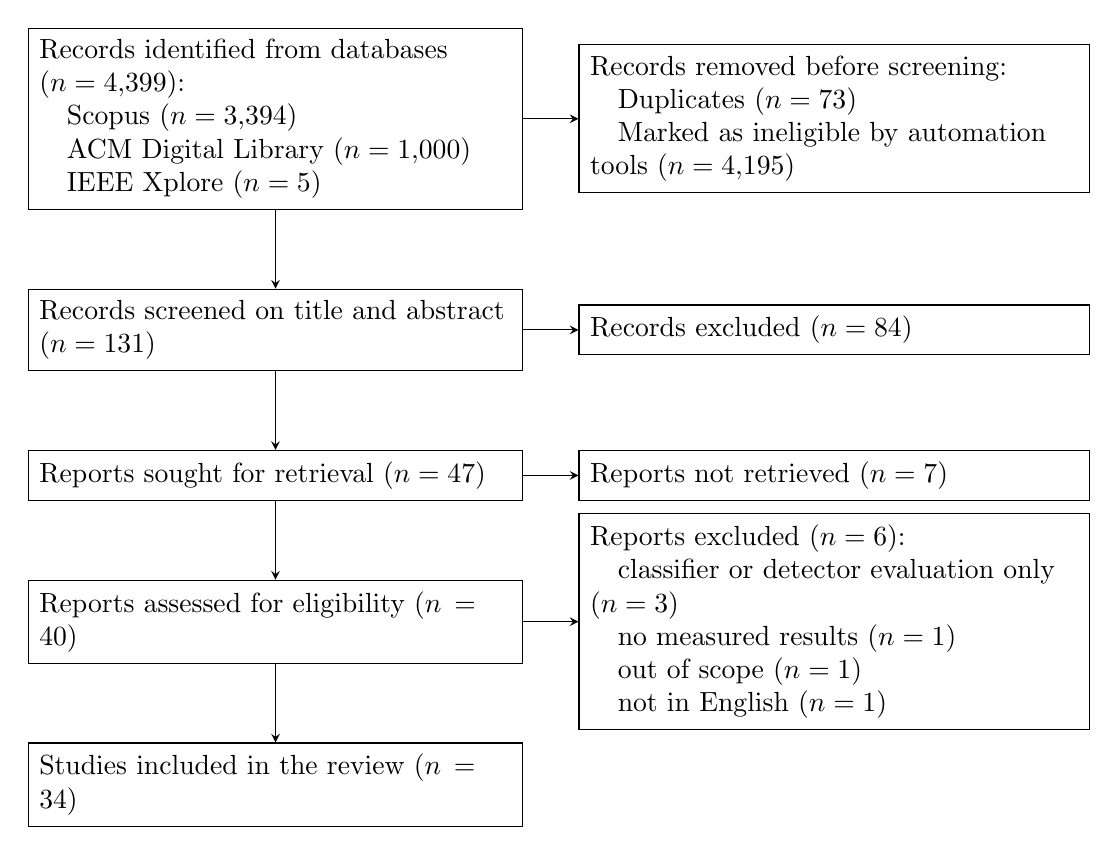
\begin{tikzpicture}[
  node distance=5mm and 7mm,
  box/.style={draw, rectangle, align=left, text width=6.0cm, inner sep=4pt},
  side/.style={draw, rectangle, align=left, text width=6.2cm, inner sep=4pt},
  arr/.style={->, >=stealth}
]
\node[box] (id) {Records identified from databases ($n=4{,}399$):\\
\quad Scopus ($n=3{,}394$)\\
\quad ACM Digital Library ($n=1{,}000$)\\
\quad IEEE Xplore ($n=5$)};
\node[side, right=of id] (rm) {Records removed before screening:\\
\quad Duplicates ($n=73$)\\
\quad Marked as ineligible by automation tools ($n=4{,}195$)};
\node[box, below=10mm of id] (scr) {Records screened on title and abstract ($n=131$)};
\node[side, right=of scr] (exta) {Records excluded ($n=84$)};
\node[box, below=10mm of scr] (sought) {Reports sought for retrieval ($n=47$)};
\node[side, right=of sought] (nr) {Reports not retrieved ($n=7$)};
\node[box, below=10mm of sought] (ass) {Reports assessed for eligibility ($n=40$)};
\node[side, right=of ass] (exft) {Reports excluded ($n=6$):\\
\quad classifier or detector evaluation only ($n=3$)\\
\quad no measured results ($n=1$)\\
\quad out of scope ($n=1$)\\
\quad not in English ($n=1$)};
\node[box, below=10mm of ass] (inc) {Studies included in the review ($n=34$)};
\draw[arr] (id) -- (scr);
\draw[arr] (id) -- (rm);
\draw[arr] (scr) -- (sought);
\draw[arr] (scr) -- (exta);
\draw[arr] (sought) -- (ass);
\draw[arr] (sought) -- (nr);
\draw[arr] (ass) -- (inc);
\draw[arr] (ass) -- (exft);
\end{tikzpicture}
\caption{PRISMA 2020 flow diagram of the systematic literature review. Citation searching was not carried out.}
\label{fig:prisma}
\end{figure}

Records marked as ineligible by automation tools are reported as a single count, as the PRISMA 2020 flow diagram allows. IEEE Xplore returned 5 records because its search was limited to open-access records (Appendix~\ref{App:scopus-search-strings}).


%-----
\chapter{Research poster layout }
\label{App:research-poster-layout}
\IfFileExists{images/poster.png}{%
\begin{figure}[H]
\centering
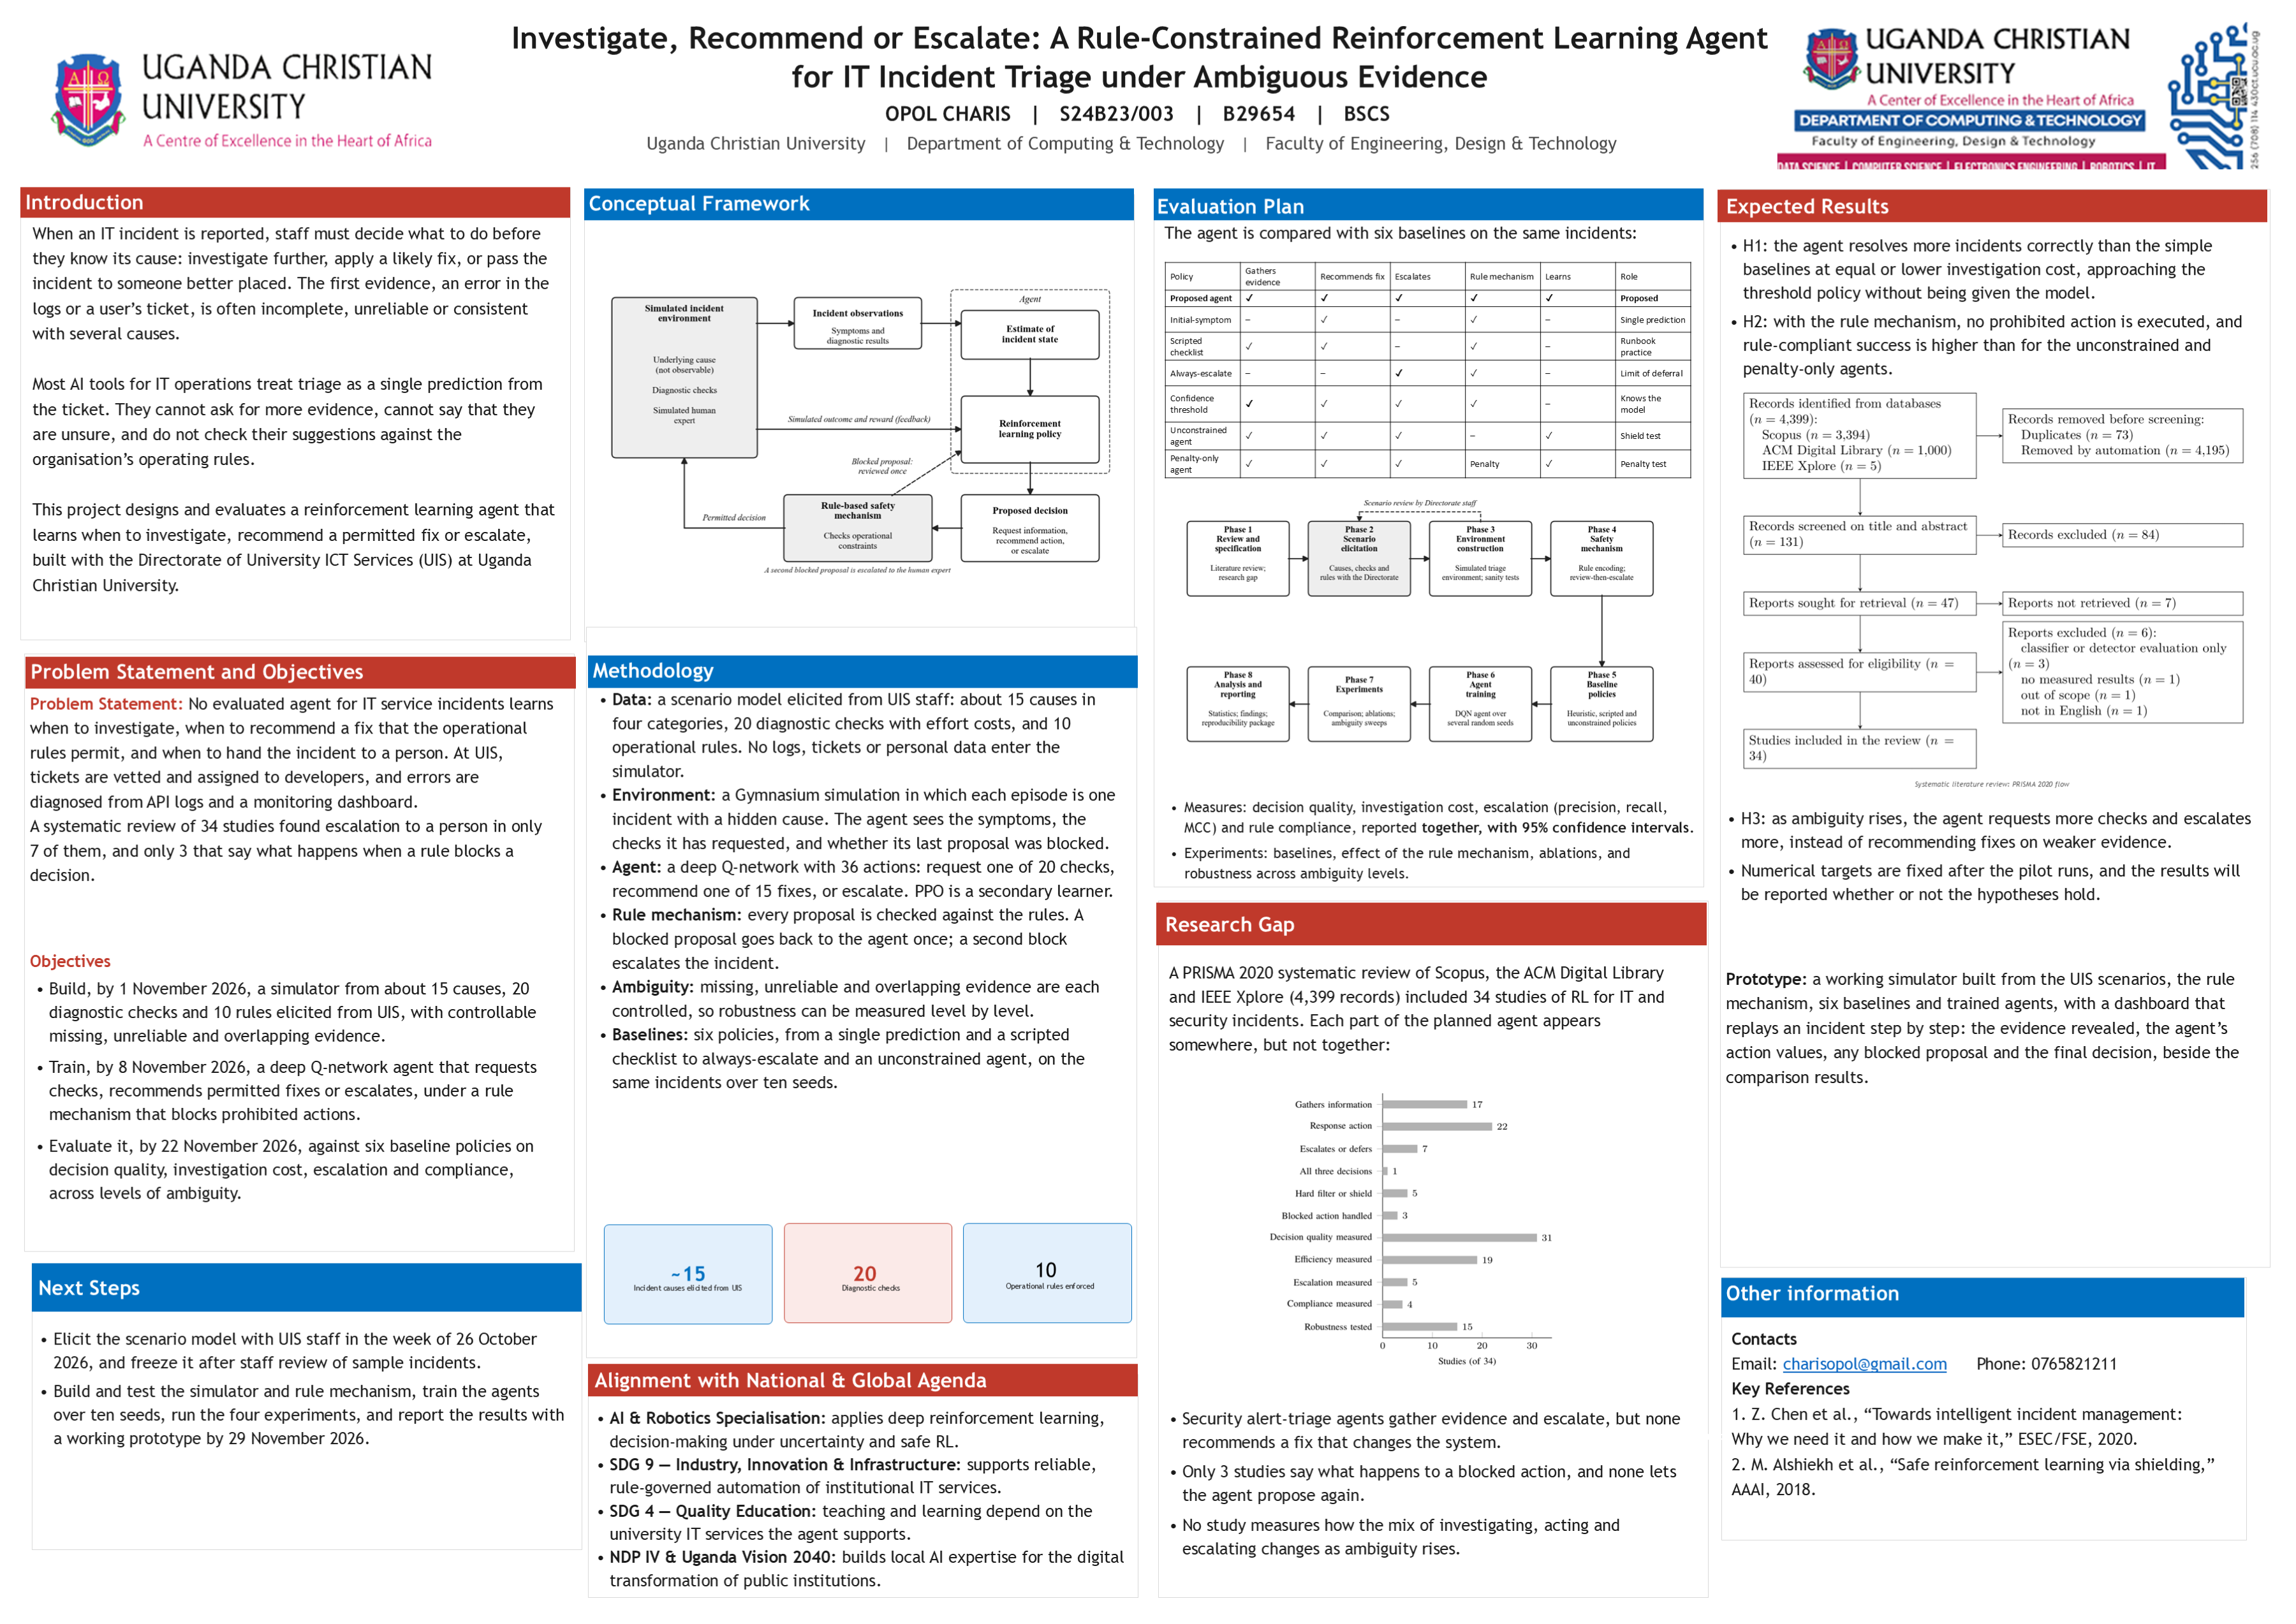
\includegraphics[width=\textwidth]{images/poster.png}
\caption{Research proposal presentation poster}
\label{fig:poster}
\end{figure}
}{\todo{Export the poster (Rule\_Constrained\_RL\_Triage\_Poster.pptx) as an image, save it as images/poster.png, and rebuild.}}


\end{appendices}


\end{document}
